\documentclass[preprint,12pt]{elsarticle}

\usepackage{amsmath,amssymb,amsfonts,mathtools}
\usepackage{amsthm}
\usepackage{algorithmic}
\usepackage{graphicx}
\usepackage{textcomp}
\usepackage{booktabs}
\usepackage{multirow}
\usepackage{array}
\usepackage{enumitem}
\usepackage{adjustbox}
\usepackage{xcolor}
\usepackage{url}
\usepackage{xspace}
\usepackage{comment}
\usepackage{tikz}
\usepackage{float}
\usepackage[caption=false]{subfig}
\usepackage{expl3}
\usepackage{xparse}
\usetikzlibrary{arrows.meta,shapes,automata,positioning,calc,fit,tikzmark,decorations.pathreplacing,decorations.markings}
% Unified monochrome figure style for the paper.
% All automata and timing diagrams use white states, black borders and black arrows.
\tikzset{
  fmstate/.style={
    circle, draw=black, fill=white, line width=0.6pt,
    minimum size=9mm, inner sep=1pt, font=\small
  },
  fmstatewide/.style={
    rounded rectangle, draw=black, fill=white, line width=0.6pt,
    minimum height=8mm, inner xsep=3pt, inner ysep=1.5pt, font=\small
  },
  fmaccept/.style={fmstate,double,double distance=1.2pt},
  fmerror/.style={fmstate,double,double distance=1.2pt,fill=gray!12},
  fmedge/.style={->,>=Stealth,line width=0.6pt},
  fmlabel/.style={font=\scriptsize,align=center,fill=white,inner sep=1.2pt},
  fminvariant/.style={font=\scriptsize,align=center},
  fmnote/.style={font=\scriptsize,align=center},
  fmtimeline/.style={->,>=Stealth,line width=0.6pt},
  fmevent/.style={circle,draw=black,fill=white,line width=0.6pt,minimum size=4.5mm,inner sep=0.5pt},
  fmreference/.style={fmevent,double,double distance=0.8pt},
  fmguide/.style={densely dashed,line width=0.45pt},
  fmbrace/.style={decorate,decoration={brace,amplitude=4pt},line width=0.5pt}
}

\DeclareUrlCommand\path{\urlstyle{tt}}
\let\pathfragile\path
\DeclareRobustCommand\path{\pathfragile}
\emergencystretch=3em
\providecommand{\href}[2]{#2}

\providecommand{\Nat}{\mathbb{N}}
\providecommand{\Real}{\mathbb{R}}
\providecommand{\CVal}{\mathsf{val}}
\providecommand{\Val}{\mathsf{val}}
\providecommand{\Inv}{\mathit{Inv}}
\providecommand{\T}{\mathcal{T}}
\providecommand{\hEventually}{\widehat{\Diamond}}
\providecommand{\hAlways}{\widehat{\Box}}
\providecommand{\optimize}{\mathsf{optimize}}
\providecommand{\export}{\mathsf{export}}
\newtheorem{theorem}{Theorem}[section]
\newtheorem{lemma}[theorem]{Lemma}
\newtheorem{proposition}[theorem]{Proposition}
\newtheorem{corollary}[theorem]{Corollary}
\newtheorem{assumption}[theorem]{Assumption}
\newtheorem{definition}[theorem]{Definition}
\journal{Journal of Systems and Software}

\InputIfFileExists{articleref}{}{}
\begin{document}
\begin{frontmatter}
\title{Supplementary Material: Verified Optimization, Export and Evaluation of a Translation from Real-Time Requirements to Timed B\"uchi Automata}
\author{Elie Fares, Jean-Paul Bodeveix, Azar Salami, Hussain Al-Aqrabi}
\begin{abstract}
This supplement contains the proof details and the material that the article summarizes: the definitions and proofs of the verified passes, the general split construction with its two policies, the conditions and proof arguments of the two certificate-checked passes, the tool details (speedups, input contract, build and artifact layout), the translator-independent synthetic evaluation, the generated-group results, and the additional evaluation material: the TChecker and generation-time tables, the UPPAAL models, the differential test, the seeded-defect study with its Rocq rejections, and the random-formula and export-policy results. References to the article are marked ``article''; all other references and numbers are to this supplement.
\end{abstract}
\end{frontmatter}

\section{Verified passes: definitions and proofs}\label{sec:passes}
\subsection{Location invariants on the trace model}
\label{sec:inv-semantics}
A location invariant maps every clock $x$ either to an upper bound
$M\in\mathbb R$, standing for the constraint $x\le M$, or to $+\infty$ (no
constraint).  We interpret automata with invariants on the extended words of
article Section~\ref{sec:model}, as we do for automata without invariants.
Along a run $r$, the automaton stays in location $r(i)$ between the events
$i-1$ and $i$, and the invariant of $r(i)$ must hold during the whole stay,
that is, at the clock values $\CVal_\rho(i,x)-\tau$ for every delay
$\tau\in[0,\Delta_{i-1}]$, where $\Delta_{i-1}=t_i-t_{i-1}$ (and at the values $\CVal_\rho(0,x)$ for the
initial location).  This is the condition of article Section~\ref{sec:model}, evaluated at
the event that ends the stay.  Since clocks increase while time elapses, an
invariant made of upper bounds holds during the stay if and only if it holds at
the event that ends it (lemma \texttt{inv\_\allowbreak{}during\_\allowbreak{}iff\_\allowbreak{}at\_\allowbreak{}event}).
For the two-sided invariants of Section~\ref{sec:forward}, a lower bound
$x\ge m$ must likewise hold during the whole stay, hence at its beginning.

\subsection{Invariant synthesis and backward propagation}
\label{sec:uppaal-invariants}\label{sec:main-invariants}
In the exported timed automaton, upper-bounded guards need invariants so that
time does not elapse past all useful outgoing transitions.  We compute location
invariants from outgoing upper bounds and propagate successor requirements
backward, using location invariants to constrain admissible time elapse as in
standard UPPAAL models~\cite{[BGD04]}.

\paragraph{Upper bound of a guard.}
For a conjunctive guard $g$ and a clock $x$, let $\mathit{ub}_x(g)$ be the
smallest bound $m$ of the constraints $x\le m$, $x<m$, and $x=m$ occurring in
$g$, and $+\infty$ if $g$ contains none.  Other constraints are ignored.  A
valuation satisfying $g$ satisfies $x\le\mathit{ub}_x(g)$.

\paragraph{Invariant synthesis.}
For a location $\ell$ with outgoing transitions
$\ell\xrightarrow{g_i,Z_i}\ell_i$, $i=1,\dots,m$, the synthesized invariant is
\[
  \mathit{Inv}(\ell)(x)=\max_{1\le i\le m}\mathit{ub}_x(g_i),
\]
with $\mathit{Inv}(\ell)(x)=+\infty$ when $\ell$ has no outgoing transition.
Thus a clock that some outgoing guard does not bound does not appear in the
invariant.  The bound is always non-strict, even when it comes from a strict
guard $x<m$: the invariant only needs to be implied by the guard of the next
transition, and strictness is kept in the guards themselves.

\begin{theorem}[Invariant synthesis]
\label{thm:inv-synthesis}
For every TBA $\mathcal A$, the automaton $\mathcal A$ with the synthesized
invariants accepts the same timed words as $\mathcal A$.
\end{theorem}

\begin{proof}
Adding invariants can only remove runs.  Conversely, let $r$ be an accepting
run on $\rho$.  At every event $i$, the transition taken from $r(i)$ is enabled,
so its guard holds at the values $\CVal_\rho(i,x)$, which are therefore at most
$\mathit{Inv}(r(i))(x)$.  By the lemma \texttt{inv\_\allowbreak{}during\_\allowbreak{}iff\_\allowbreak{}at\_\allowbreak{}event}, the invariant of $r(i)$ holds during
the whole stay.  (Rocq: \texttt{add\_\allowbreak{}invariants\_\allowbreak{}correct}.)
\end{proof}

\paragraph{Backward propagation.}
One propagation step strengthens every transition
$\ell\xrightarrow{g,Z}\ell'$ with the invariant of its target after the
resets:
\[
  g := g\wedge\mathit{Inv}(\ell')[Z:=0],
\]
where $\mathit{Inv}(\ell')[Z:=0]$ replaces every bound $x\le M$ on a reset clock
$x\in Z$ by the constant constraint $0\le M$, that is, by $\top$ if $M\ge0$ and
by $\bot$ otherwise.  Invariants are then synthesized again from the
strengthened guards.

\begin{theorem}[Backward propagation]
\label{thm:propagation}
For every TBA $\mathcal A$ and every $n\in\Nat$, the automaton obtained by
$n$ propagation steps accepts the same timed words as $\mathcal A$.
\end{theorem}

\begin{proof}
Strengthening guards can only remove runs.  Conversely, consider an accepting
run that takes $\ell\xrightarrow{g,Z}\ell'$ at event $i$ and then a transition
$\ell'\xrightarrow{g',Z'}\ell''$ at event $i+1$.  The second guard holds at event
$i+1$, so the values at that event are bounded by $\mathit{Inv}(\ell')$.  Clock
consistency gives $\CVal_\rho(i+1,x)=\Delta_i$ for $x\in Z$ and
$\CVal_\rho(i+1,x)=\CVal_\rho(i,x)+\Delta_i\ge\CVal_\rho(i,x)$ otherwise; hence
the strengthened guard $g\wedge\mathit{Inv}(\ell')[Z:=0]$ holds at event $i$.
The argument uses clock consistency, so the theorem is stated on timed words.
(Rocq: \texttt{propagate\_\allowbreak{}accepts} and
\texttt{propagate\_\allowbreak{}n\_\allowbreak{}accepts}.)
\end{proof}

Each round of the optimization pipeline of article Section~\ref{sec:main-pipeline}
applies one propagation step.  The tool repeats the rounds until the
automaton is structurally equal to the previous one, as an OCaml value, or
until 50 rounds have been performed; the bound guarantees termination, and the
theorem holds for every number of steps, whether or not a fixed point is
reached. On the 29 completed optimizer inputs, the greatest observed number
of changed rounds is six (R6).
The invariant computation at one location is summarized in Figure~\ref{fig:main-inv-unified}.

\begin{figure}[t]
\centering
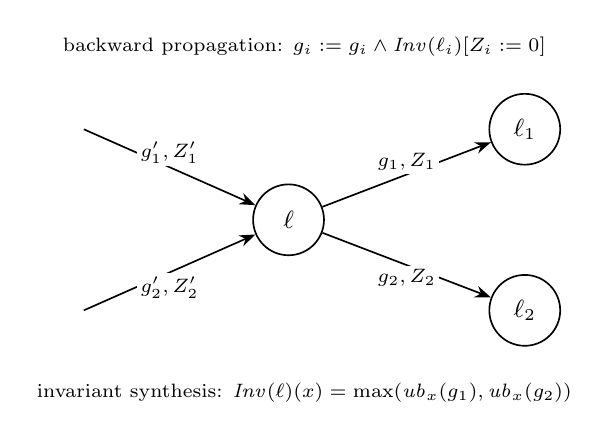
\begin{tikzpicture}[node distance=20mm]
  \node[fmstate] (L) at (0,0) {$\ell$};
  \node[fmstate] (S1) at (3.0,1.15) {$\ell_1$};
  \node[fmstate] (S2) at (3.0,-1.15) {$\ell_2$};
  \coordinate (P1) at (-2.6,1.15);
  \coordinate (P2) at (-2.6,-1.15);
  \draw[fmedge] (P1) -- node[fmlabel,above] {$g'_1,Z'_1$} (L);
  \draw[fmedge] (P2) -- node[fmlabel,below] {$g'_2,Z'_2$} (L);
  \draw[fmedge] (L) -- node[fmlabel,above] {$g_1,Z_1$} (S1);
  \draw[fmedge] (L) -- node[fmlabel,below] {$g_2,Z_2$} (S2);
  \node[fmnote] at (0.20,2.20) {backward propagation: $g_i:=g_i\land \mathit{Inv}(\ell_i)[Z_i:=0]$};
  \node[fmnote] at (0.20,-2.20) {invariant synthesis: $\mathit{Inv}(\ell)(x)=\max(\mathit{ub}_x(g_1),\mathit{ub}_x(g_2))$};
\end{tikzpicture}

\caption{Invariant computation at one location. Successor invariants strengthen outgoing
guards; upper bounds of the resulting guards resynthesize the source
invariant. Reset sets determine which target-clock constraints become
constant.}
\label{fig:main-inv-unified}
\end{figure}

\paragraph{Example.}
We illustrate the algorithm on the automaton of Fig.~\ref{fig:inv-example},
which contains a two-location cycle $\ell_1\to\ell_2\to\ell_1$ and a self-loop
at $\ell_2$.  It has one clock $x$, the initial location $\ell_0$, and the
transitions
\[
\begin{aligned}
&\ell_0 \xrightarrow{a,\;Z=\{x\}} \ell_1,\quad
 \ell_1 \xrightarrow{b,\;x\le 2,\;Z=\emptyset} \ell_2,\\
&\ell_2 \xrightarrow{c,\;\top,\;Z=\emptyset} \ell_1,\quad
 \ell_2 \xrightarrow{d,\;x\le 1,\;Z=\emptyset} \ell_2.
\end{aligned}
\]
The edge $\ell_1\xrightarrow{b}\ell_2$ requires $x\le2$, and the self-loop at
$\ell_2$ requires the tighter bound $x\le1$.

\begin{figure}[t]
\centering
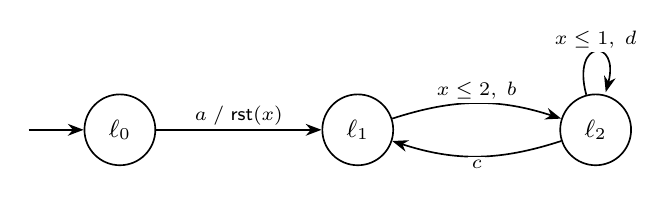
\begin{tikzpicture}[node distance=21mm]
  \node[fmstate] (l0) {$\ell_0$};
  \node[fmstate,right=of l0] (l1) {$\ell_1$};
  \node[fmstate,right=of l1] (l2) {$\ell_2$};
  \draw[fmedge] ([xshift=-7mm]l0.west) -- (l0.west);
  \draw[fmedge] (l0) -- node[fmlabel,above] {$a\;/\;\mathsf{rst}(x)$} (l1);
  \draw[fmedge] (l1) to[bend left=18] node[fmlabel,above] {$x\le2,\;b$} (l2);
  \draw[fmedge] (l2) to[bend left=18] node[fmlabel,below] {$c$} (l1);
  \draw[fmedge] (l2) edge[loop above] node[fmlabel] {$x\le1,\;d$} (l2);
\end{tikzpicture}

\caption{Automaton used to illustrate invariant propagation, with one clock $x$
and actions $a$--$d$.  Edges are labeled ``guard, action / resets'' (the guard
is omitted when it is $\top$); only the edge $\ell_0\to\ell_1$ resets $x$.  The
incoming arrow marks the initial location; acceptance plays no role here.  The
computed fixed point is $\mathit{Inv}(\ell_1)=\mathit{Inv}(\ell_2)=(x\le2)$.}
\label{fig:inv-example}
\end{figure}

\begin{enumerate}
\item \emph{Synthesis.}  $\mathit{Inv}(\ell_1)(x)=\mathit{ub}_x(x\le2)=2$.  At
$\ell_2$, $\mathit{Inv}(\ell_2)(x)=\max(1,+\infty)=+\infty$, because the
transition toward $\ell_1$ does not bound $x$.  At $\ell_0$, the only outgoing
guard is $\top$, so $\mathit{Inv}(\ell_0)(x)=+\infty$.

\item \emph{Propagation.}  The transition
$\ell_2\xrightarrow{c,\;Z=\emptyset}\ell_1$ becomes guarded by
$\top\wedge\mathit{Inv}(\ell_1)=(x\le2)$.  The transition
$\ell_0\xrightarrow{a,\;Z=\{x\}}\ell_1$ receives $(0\le2)\equiv\top$ and is
unchanged.

\item \emph{Synthesis.}  At $\ell_2$, the outgoing guards are now $x\le1$ and
$x\le2$, so $\mathit{Inv}(\ell_2)(x)=\max(1,2)=2$.

\item \emph{Propagation.}  The transition $\ell_1\xrightarrow{b,\;x\le2}\ell_2$
receives $x\le2$, which it already contains, and the self-loop at $\ell_2$
receives $x\le2$, which is implied by $x\le1$.  Nothing changes.
\end{enumerate}
The fixed point is $\mathit{Inv}(\ell_0)=\top$ and
$\mathit{Inv}(\ell_1)=\mathit{Inv}(\ell_2)=(x\le2)$.  While the automaton
remains in the cycle $\ell_1\leftrightarrow\ell_2$, the clock $x$ cannot exceed
$2$, and at every reachable valuation at least one outgoing transition of the
current location is enabled.  The invariants do not remove every blocking
behavior: since $x$ is never reset in the cycle, time is blocked once $x=2$.
They make the upper bounds of the property automaton explicit, and
Theorems~\ref{thm:inv-synthesis} and~\ref{thm:propagation} guarantee that they
do not change its language.

\subsection{Forward propagation of lower bounds and simplification}
\label{sec:forward}\label{sec:main-forward}
\paragraph{Entry bounds.}
Dually, for a transition $t=\ell\xrightarrow{g,Z}\ell'$ and a clock $x$, the
\emph{entry bound} of $x$ along $t$ is $0$ if $x\in Z$ and otherwise the
largest bound $\mathit{lb}_x(g)$ of the constraints $x\ge m$, $x>m$, and $x=m$
of $g$, if any.  The entry bound of $x$ at a location $\ell'$ is the minimum of
the entry bounds of $x$ along the transitions entering $\ell'$; for the initial
location, the initial entry, with bound $0$, also counts.  If some entering
transition gives no bound on $x$, the clock $x$ has no entry bound at $\ell'$.
Since clocks are nonnegative and do not decrease while time elapses, every
clock with entry bound $m$ at $\ell'$ satisfies $x\ge m$ during every stay in
$\ell'$.

\paragraph{Forward propagation.}
The forward step adds $x\ge m$ to the guard of every transition leaving
$\ell'$, for every clock $x$ with entry bound $m$ at $\ell'$ (Rocq:
\texttt{forward\_\allowbreak{}accepts}).  The entry bounds can also be read as lower-bound
invariants: the two-sided automaton that carries the synthesized upper-bound
invariants and the entry bounds as lower-bound invariants accepts the same
timed words (\texttt{add\_\allowbreak{}two\_\allowbreak{}sided\_\allowbreak{}invariants\_\allowbreak{}accepts}).  UPPAAL
rejects lower-bound invariants, and their only role is to make infeasible
transitions visible: after forward and backward propagation, a transition whose
source location bounds a clock from below and whose target bounds it from above
carries both bounds in its guard.

\paragraph{Simplification.}
Three simplifications follow.  First, a transition whose guard contains
contradictory constraints is removed: a lower bound and an upper bound on the
same clock with $u<l$, or with $u=l$ and one of them strict, or an upper bound
$x\le u$ with $u<0$ or $x<u$ with $u\le0$.  Such a transition is never enabled (Rocq:
\texttt{remove\_\allowbreak{}contradictory\_\allowbreak{}accepts}).  Second, the transitions
leaving a non-initial location that has no entering transition
are removed: such a location never occurs on a run after position~$0$ (Rocq:
\texttt{remove\_\allowbreak{}unreachable\_\allowbreak{}accepts}).  The iteration of the pipeline
removes chains of such locations one step at a time.  A location whose only
entering transitions are self-loops keeps them, but it is unreachable from
the initial location; the tool counts and prints only the locations
reachable from the initial one and their transitions.  Third, a transition whose
action label is unsatisfiable, because it requires two different actions or an
action and its negation, is removed (Rocq:
\texttt{remove\_\allowbreak{}unsat\_\allowbreak{}accepts}).  Such labels arise when the
translator receives an action $a$ and the atom $\neg a$ of $\T(f)$ as independent
propositions (the tool option \texttt{-indep-neg} of the translation article;
its default negates the atom for $a$, which avoids most of them) or when a cube
requires two different actions; removing them also enables clock merging, since the resets of a
transition that can never be taken would otherwise prevent it.

\subsection{Dead resets and merging of synchronously reset clocks}
\label{sec:dead-merge}\label{sec:main-dead-merge}
\paragraph{Dead resets.}
A clock $x$ is \emph{live} at a location $\ell$ if some transition that tests
$x$ in its guard can be taken from $\ell$, possibly after other transitions.
The live locations are computed as a backward closure, along all
transitions, from the sources of the transitions that test $x$; the other
locations are \emph{dead} for $x$.  Since the correctness of the pass does
not depend on how this closure is computed, the pass checks the two
properties that the proof uses, namely that no transition leads from a dead
location to a live one and that none tests $x$ from a dead location, and then removes $x$ from the reset sets of the
transitions that enter a dead location.  After such a transition, the value of
$x$ is never read again, so whether it is reset does not matter.  The proof
builds, from every accepted extended word, an extended word that differs only
in the reset decisions of $x$, and conversely (Rocq:
\texttt{remove\_\allowbreak{}dead\_\allowbreak{}resets\_\allowbreak{}clock\_\allowbreak{}accepts}).  The pass is applied
to every clock (\texttt{remove\_\allowbreak{}dead\_\allowbreak{}resets\_\allowbreak{}accepts}).

\paragraph{Synchronous clocks.}
The verified translation shares the clock of syntactically identical timed
subformulas.  Clocks of \emph{different} subformulas can also be merged when
they are reset synchronously.  Two clocks $x\neq y$ are \emph{mergeable} if
\begin{enumerate}[label=(\roman*)]
  \item every transition resets $x$ if and only if it resets $y$;
  \item no transition enters the initial location; and
  \item every transition leaving the initial location resets $x$ and does not
        test it.
\end{enumerate}
Then, after the first event, $x$ and $y$ always have the same value, and every
test of $x$ can be replaced by the same test on $y$ (Rocq:
\texttt{merge\_\allowbreak{}accepts}).  The condition is checked by a Boolean function
proved to imply it, and the pass tries all pairs of reset clocks
(\texttt{merge\_\allowbreak{}all\_\allowbreak{}accepts}).  The merged clock $x$ is no longer tested,
so its remaining resets are removed by the dead-reset pass in the next round.
This verified merging is restricted to synchronously reset clocks; merging
clocks whose values coincide for other reasons is not covered.

\subsection{Normalization of guards}
\label{sec:normalize}
Backward and forward propagation add constraints to guards.  Every time a
guard is strengthened, it is \emph{tightened}: a constraint implied by another
constraint of the same guard on the same clock is dropped, so that a guard
keeps at most one lower bound and one upper bound per clock (an equality
counting as both); for instance, $x\le5\land x<2$ becomes $x<2$.  The
implication test compares bounds and strictness, and is proved sound (Rocq:
\texttt{tighten\_\allowbreak{}holds}).  Normalization tightens every guard and also
removes the lower bounds $x\ge m$ with $m\le0$ and $x>m$ with $m<0$, which every
clock value satisfies; it is needed after the merging of clocks, which renames
constraints.  The removal of trivial lower bounds relies on the nonnegativity
of clock values, so the theorem is stated on timed words (Rocq:
\texttt{normalize\_\allowbreak{}accepts}).

\subsection{Merging of transitions and of locations}
\label{sec:merge-ts}\label{sec:main-merge-ts}
\paragraph{Transitions.}
Two transitions with the same source, target, and resets are merged when the
union of their enabling conditions is again a conjunction.  A transition is
removed when another transition with the same source, target, and resets is
\emph{weaker}, that is, when its label and guard imply those of the other
transition, constraint by constraint (subsumption).  Two transitions
whose labels, or guards, differ only by a literal and its negation, such as
$p$ and $\neg p$, $x<2$ and $x\ge2$, or $x\le5$ and $x>5$, are replaced by one
transition without that literal (resolution).  The pass preserves the language
because every enabled transition has an enabled counterpart with the same
source and target, and conversely (Rocq: \texttt{merge\_\allowbreak{}trans\_\allowbreak{}accepts}).
The other unions are disjunctive; they are formed by the export
(article Section~\ref{subsec:split-construction}).

\paragraph{Locations.}
A location $\ell'$ is merged into a location $\ell$ when both are accepting or
both are not, and when (i) every transition leaving $\ell'$ is subsumed by a
transition leaving $\ell$, and (ii) every transition leaving $\ell$ is subsumed
by one leaving $\ell'$.  A transition $u$ subsumes $t$ when it has a weaker
label, the same resets, the same target once $\ell'$ is replaced by $\ell$, and
every constraint of its guard is implied by a constraint of the guard of $t$.
In (i) the guard of $t$ is conjoined with the \emph{entry invariant} of
$\ell'$: the lower bounds $x\ge m$ that hold at every visit of $\ell'$.  They
are the entry bounds of Section~\ref{sec:forward}, except that a self-loop of
$\ell'$ that does not reset $x$ is ignored, because it preserves a lower bound
(Rocq: \texttt{entry\_\allowbreak{}lb\_\allowbreak{}loop\_\allowbreak{}sound}).
Both orders of a pair are tried.  The transitions entering
$\ell'$ are redirected to $\ell$, and those leaving $\ell'$ are removed.  A run
of the original automaton becomes a run of the merged one by replacing $\ell'$
by $\ell$, using (i) and the invariant; conversely, a run of the merged
automaton is followed in the original one, taking in $\ell'$ a transition that
subsumes the one taken in $\ell$, by (ii)
(Rocq: \texttt{merge\_\allowbreak{}states\_\allowbreak{}all\_\allowbreak{}accepts}; ``state'' in a Rocq name
means location).  The condition on the B\"uchi marking is necessary: merging
an accepting location with a non-accepting one would accept runs that visit only the latter infinitely
often.


\section{General split construction and the two split policies}
\subsection{General split construction and preservation}
\label{subsec:split-detail}
Let $U_1,\dots,U_r$ be the irredundant conjunctions of non-strict upper bounds
of a disjunctive invariant; the construction makes one copy per $U_k$. At
entry valuation $v$, the largest delay admitted by $U_k$ is
\[
 d_k(v)=\min_{(x,b)\in U_k}(b-v(x)),
 \qquad d_k(v)=+\infty\text{ when }U_k=\varnothing.
\]
The entry predicate for copy $k$ is
\[
 G_k(v)\equiv U_k(v)\ \land\ \bigwedge_{\ell=1}^{r} d_\ell(v)\le d_k(v).
\]
Thus a copy is admitted only if its invariant holds at entry and no other
copy permits a strictly longer stay. To encode the comparison without
introducing a new clock, the implementation chooses an upper bound
$y\le b_y$ in $U_\ell$ and requires it to be reached no later than every
bound $x\le b_x$ in $U_k$. This gives $v(x)-v(y)\le b_x-b_y$. The
disjunction over possible minimizing bounds is represented in DNF. When some
$U_\ell$ is empty, $d_\ell=+\infty$ and the comparison $d_\ell\le d_k$ holds only for an
empty $U_k$; the encoding then reduces to the constants true and false rather than to a choice of bound. An
incoming edge reset set $Z$ is handled by substituting zero for clocks in
$Z$ before conjoining $G_k$ with the edge guard: a difference constraint
with two reset clocks becomes a constant test, one reset clock gives a unary
comparison, and no reset clock leaves a diagonal constraint.

The copy invariants are generated from the outgoing transition guards. If
$\operatorname{ub}(c)$ extracts the non-strict unary upper bounds from a
conjunctive guard clause $c$, the coverage contract is
\[
\begin{gathered}
\forall t\in\operatorname{Out}(q),\ \forall c\in\operatorname{DNF}(g_t),\\
\exists U\in\mathcal U(q):\quad \operatorname{ub}(c)\Rightarrow U.
\end{gathered}
\]
Here $t$ has source $q$ and guard $g_t$; implication means that every
valuation satisfying all extracted upper bounds also satisfies every bound
in $U$. The Rocq lemma \texttt{disj\_inv\_cover} proves this coverage for
the deduplicated list $\mathcal U(q)$; it is an internal construction
invariant, not a precondition imposed on callers. At the endpoint of any taken
transition, the selected guard clause therefore entails a generated
upper-bound conjunction. Since clocks only increase during the stay, those
non-strict upper bounds also hold at each earlier valuation. This coverage
argument is the key completeness condition for both the verified split and
the all-copy comparison below.

All copies inherit the original location's accepting mark. No silent edge is
added, and the proof relates runs by projecting each copy back to its
original location. Thus repeated visits to an accepting location correspond
to repeated visits to accepting copies, preserving B\"uchi acceptance. In
Rocq, \texttt{split\_accepts} proves timed-word preservation when the input
invariant function is everywhere absent; \texttt{of\_tba} establishes that
precondition for the TBA export pipeline. The split invariant is absent or
one conjunction per location by \texttt{split\_inv\_conjunctive}; the full
export shape is established by \texttt{export\_guards\_conjunctive} and
\texttt{export\_invariants\_conjunctive}. These are the internal
representation theorems; the XML printer is not verified.

The optimized automaton has normalized conjunctive guards. Export first merges transitions that agree on source, target, event label, and resets, placing their guards into a disjunction. The location invariant is then represented by disjunctions of conjunctions of upper bounds. UPPAAL-oriented output requires each such invariant to be conjunctive because its location syntax admits a conjunction of clock conditions, so a disjunction must be encoded by a structural transformation~\cite{[BGD04]}. Retaining a disjunction directly would not meet the target representation.

Every incoming edge is replicated to each regular target copy and conjoined with its reset-adjusted entry predicate; outgoing edges are replicated from every copy. This replication is essential: copying only the location and assigning incoming edges to one arbitrarily chosen disjunct can truncate a stay and lose a timed word. The initial location uses a dedicated invariant-free copy because the first timed-word event has no incoming edge.

The representation cost follows directly from this construction. Let
$K=\mathsf{kp}(D)$ be the number of source-copy slots used by the
implementation and let $r(q)$ be the number of regular invariant copies of
location $q$. Before guard explosion, each original edge $t$ contributes
$K\,r(\mathit{tgt}(t))$ split transition records. After guard explosion,
the corresponding explicit-edge count is
\[
 E_{\mathrm{split}}=\sum_{t\in T}K\sum_{k<r(\mathit{tgt}(t))}
 \left|\operatorname{DNF}\!\left(g_t\land
   \operatorname{subst}_{Z_t}(G_k)\right)\right|.
\]
This count is taken before later normalization and pruning. It exposes two
sources of growth: the number of invariant copies at the target and the DNF
size of reset-adjusted entry guards. It is a structural count of the
construction, not a complexity bound for the entire exporter.

Language preservation does not require selecting a copy with the longest
admissible residence interval. We therefore mechanized a second policy,
called the \emph{all-copy split}: it retains the same conjunctive invariant
copies, invariant-free initial copy, and accepting marks, but sends every
incoming transition to every regular target copy with its original guard and
reset set. It has no reset-adjusted entry predicate. The copy coverage
property \texttt{disj\_inv\_cover} is established inside the Rocq
construction, not assumed from an external parser.

\begin{theorem}[All-copy split preservation]
Let $D$ be an input DTA with no pre-existing location invariants. The
all-copy construction computes its upper-bound disjunctions and proves
\texttt{disj\_inv\_cover} internally. Then the all-copy variant and $D$
accept the same timed words.
\end{theorem}
\begin{proof}
For soundness, project a run of the split automaton from each copy to its
original location. Each copied transition keeps its original label, guard,
and resets. The regular copies add their associated upper-bound conjuncts,
but the input automaton has no location invariants, so projection forgets
only this additional condition. The initial copy has no invariant, as required
by the input contract. Accepting marks are inherited, so infinitely many
accepting visits are preserved.

For completeness, fix an accepting run of $D$. At each noninitial location
occurrence, consider the outgoing transition used by that run and a DNF
clause $c$ of its guard that holds at the event ending the stay. By
\texttt{disj\_inv\_cover}, some copy invariant $U_k$ is implied by the
upper-bound part of $c$. Hence $U_k$ holds at that ending event. Each atom
of $U_k$ is a non-strict upper bound, so it also holds at every earlier
valuation in the stay: clocks only increase during delay, and resets occur
at its beginning. Thus copy $k$ satisfies its invariant throughout this
stay. The preceding transition is available to every regular target copy,
and every outgoing transition is available from each source copy. Choosing
copy $k$ on entry therefore lifts this occurrence of the run. The initial
occurrence uses the dedicated invariant-free copy. Making this choice at
each occurrence preserves the event sequence and resets; inherited
accepting marks give infinitely many accepting visits in the lifted run.
The two inclusions establish language equality.
\end{proof}

\begin{theorem}[Maximal-delay split preservation]
Let $D$ be an input DTA with no pre-existing location invariants. The
maximal-delay variant (Rocq: \texttt{split\_accepts}) and $D$ accept the same timed words.
\end{theorem}
\begin{proof}
Soundness is the projection argument of the previous proof: every copied transition keeps its
label and resets, and its guard is the original guard conjoined with an entry predicate, so
the projection of a run of the split automaton is a run of $D$. For completeness, fix an
accepting run of $D$ and a stay at a noninitial location $q$, entered with valuation $v$
(after the resets of the incoming edge) and left after a delay $\Delta$ by a transition whose guard
clause $c$ holds at the end of the stay. By \texttt{disj\_inv\_cover} there is $k^*$ with
$\operatorname{ub}(c)\Rightarrow U_{k^*}$, so $U_{k^*}$ holds at the end of the stay and
$b-v(x)\ge\Delta$ for every $(x,b)\in U_{k^*}$, that is, $d_{k^*}(v)\ge\Delta$. Let $k$ maximize $d_k(v)$
(\texttt{best\_spec}; ties are all admissible, and $+\infty$ is allowed). Then $d_k(v)\ge d_{k^*}(v)\ge\Delta$,
so every bound of $U_k$ still holds at the end of the stay and, being non-strict upper bounds on increasing
clocks, throughout it; and $G_k(v)$ holds by the choice of $k$, so the incoming edge, whose guard is conjoined with the
reset-adjusted predicate $G_k$, can enter copy $k$. The outgoing transition is available from every
copy. Making this choice at each occurrence lifts the run; accepting marks are inherited, and
the initial occurrence uses the invariant-free initial copy. The two inclusions give language equality.
\end{proof}

The maximal-delay policy establishes a stronger local copy-choice property:
at a given entry valuation, every admitted copy has an admissible residence
duration at least as long as that of any other copy. The helper lemma
\texttt{best\_spec} proves maximization, including $+\infty$ for an empty
conjunction; ties remain admissible. This is neither global deadlock
freedom nor a theorem about time divergence. Compared with all-copy
replication, maximal-delay entry selection can introduce clock-difference
constraints and more DNF clauses, while it may avoid entering copies that
expire strictly earlier. The measured alternatives exhibit a trade-off
(Table~\ref{tab:split-comparison}): on a two-clock example all-copy uses four
more explicit edges but fewer guard atoms and no diagonal constraints; on a
six-branch family both produce 68 edges, while all-copy uses fewer guard
atoms and no diagonal constraints. All-copy is faster on the small case and
slower on the six-branch case in these measurements. These are synthetic
measurements, not a general performance ordering. The default remains the existing
maximal-delay transformation; all-copy is separately verified and exposed
for comparison.

\begin{table*}[t]
\centering
\caption{Measured split policies on direct synthetic TBAs. ``Two-clock'' is the
\texttt{disjunctive\_invariant\_export} record of Table~\ref{tab:synthetic-tba}
and ``six-branch'' the disjunctive-invariant family at $k=6$ of
Table~\ref{tab:parameterized-synthetic}. Locations are graph-reachable
locations. Times are means over 200 in-memory export calls.}
\label{tab:split-comparison}
\scriptsize
\begin{tabular}{@{}llrrrrr@{}}
\toprule
Input & Policy & Reach. loc. & Edges & Guard atoms & Diagonal atoms & Time (ms)\\
\midrule
Two-clock & Maximal delay & 3 & 6 & 12 & 6 & 0.831\\
Two-clock & All-copy & 3 & 10 & 8 & 0 & 0.712\\
Six-branch & Maximal delay & 5 & 68 & 320 & 204 & 15.990\\
Six-branch & All-copy & 5 & 68 & 64 & 0 & 28.731\\
\bottomrule
\end{tabular}
\end{table*}


\section{Certificate-checked passes: conditions and proofs}\label{sec:checked-detail}
\subsection{Scheme and trusted base}
Both passes have the same structure. An untrusted OCaml procedure (the \emph{certifier}) returns a certificate; a boolean function written in Rocq and extracted tests local conditions on it; and a \emph{try} function applies the transformation if the test returns \path{true} and returns its input otherwise. The preservation theorem is stated for an arbitrary certificate, in the form
\[
\forall\, \mathsf{cert}\ \mathcal A,\quad \mathcal L(\mathsf{pass}(\mathsf{cert},\mathcal A))=\mathcal L(\mathcal A),
\]
where the pass is \path{prune_pass} or \path{alloc_pass} and \path{prune_certifier}, \path{certifier} are the function types of the certifiers. The proof never inspects how a certificate was found, so a wrong certifier can lower the quality of the result and cannot change its language. Nothing is added to the axioms of the rest of the development. The proofs are in \path{MTL_to_TBA_DomPrune.v} (pruning and \path{split_cells}) and \path{MTL_to_TBA_ClockAlloc.v} (clock reuse), and the composition theorems are in \path{MTL_to_TBA_CheckedPasses.v}.

\subsection{Removal of dominated transitions}\label{sec:prune-detail}
\paragraph{Cells of letters.} Let $\mathit{men}(\mathcal A)$ be the actions that occur in a label of $\mathcal A$ (\path{mentioned}). A \emph{cell} is either $\mathsf{Some}\,a$ with $a\in\mathit{men}(\mathcal A)$ or $\mathsf{None}$, which stands for every action outside $\mathit{men}(\mathcal A)$; \path{cells} lists them and \path{cell_of} maps an action to its cell. A label is a conjunction of literals over actions, and with one action at each position \path{label_at} decides it on a cell: a positive literal $a$ holds on $\mathsf{Some}\,a$ only, and a negative literal $\neg a$ holds on every cell except $\mathsf{Some}\,a$. Lemma \path{label_at_iff} states that a label of $\mathcal A$ holds on an action $p$ exactly when it holds on the cell of $p$. Dominance can therefore be tested on finitely many cells and not on all letters.

\paragraph{The certificate.} A certificate for $\mathcal A$ consists of a predicate $\mathit{keep}$ on transitions, a relation $\mathit{sim}$ on locations, and, for every location $q$, two lists of clocks $\mathit{live}(q)$ and $\mathit{lle}(q)$. The pruned automaton \path{prune_trans} has the same locations, initial location and accepting set as $\mathcal A$ and only the transitions that satisfy $\mathit{keep}$.

\paragraph{The checker.} \path{prune_ok} returns \path{true} iff $\mathit{sim}(q_0,q_0)$ for the initial location $q_0$ and, for all locations $q_1,q_2$ with $\mathit{sim}(q_1,q_2)$:
\begin{enumerate}[label=(P\arabic*),leftmargin=*,itemsep=0pt]
  \item if $q_2$ is accepting then $q_1$ is accepting;
  \item for every cell $c$ and every transition $t_2$ out of $q_2$ whose label holds on $c$, there is a transition $t_1$ out of $q_1$ (\path{dom_step}) such that
  \begin{enumerate}[label=(\alph*),itemsep=0pt]
    \item $\mathit{keep}(t_1)$, and the label of $t_1$ holds on $c$;
    \item the guard of $t_2$ implies the guard of $t_1$ (\path{guard_implied}), and every atom of the guard of $t_1$ has its clock in $\mathit{live}(q_1)$, or is an upper bound ($<$ or $\le$) on a clock of $\mathit{lle}(q_1)$ (\path{guard_item_ok});
    \item (\path{flow_ok}) every clock $x\in\mathit{live}(\mathit{tgt}(t_1))$ is reset by both $t_1$ and $t_2$, or by neither and then $x\in\mathit{live}(q_1)$; every clock $x\in\mathit{lle}(\mathit{tgt}(t_1))$ is reset by $t_1$, or is reset by neither and $x\in\mathit{lle}(q_1)\cup\mathit{live}(q_1)$;
    \item $\mathit{sim}(\mathit{tgt}(t_1),\mathit{tgt}(t_2))$.
  \end{enumerate}
\end{enumerate}
The test is a finite conjunction over locations, cells and transitions. It is written with a lazy conjunction (\path{land}) because the extracted code of \path{andb} evaluates both arguments, and the check runs on automata with thousands of transitions; \path{dom_step_spec} and \path{prune_ok_spec} give the propositional reading above.

\paragraph{Meaning of $\mathit{live}$ and $\mathit{lle}$.} For two runs, one of $\mathcal A$ at a location $q_2$ and one of the pruned automaton at a location $q_1$ with $\mathit{sim}(q_1,q_2)$, the clocks of $\mathit{live}(q_1)$ will have \emph{equal} values and those of $\mathit{lle}(q_1)$ will have a value in the second run that is \emph{less than or equal} to the value in the first. Equality is needed for guards of any shape; the order is enough for upper bounds, since the run of $t_1$ satisfies $x\le c$ whenever the run of $t_2$ does and its value of $x$ is not larger. The resets of the two transitions may differ on a clock that is dead after the step, which is what lets $t_1$ dominate a transition with a different reset set; this is the difference with syntactic subsumption (article Section~\ref{sec:post}), which requires the same target and the same resets.

\paragraph{The invariant.} Given a run $\pi$ of $\mathcal A$ on an extended word $\rho$ (positions $0,1,\dots$ with the actions, delays and clock values of $\rho$), the proof builds, by recursion on $i$, a run of the pruned automaton: \path{T2} $i$ is the transition of $\mathcal A$ taken at position $i$; \path{T1} $i$ $q$ is, by \path{pick}, the transition that \path{prune_ok_spec} provides for $q$, the cell of the action at $i$ and \path{T2} $i$; \path{qs} $i$ is the location reached, with $\mathsf{qs}\,0=q_0$; and the valuations \path{dpval} are those obtained by applying the resets of the chosen transitions to the delays of $\rho$. The record \path{dp_inv} states four facts at each position $i$:
\begin{gather*}
\mathit{sim}(\mathsf{qs}_i,\pi_i)\ \wedge\ \mathsf{qs}_i<|\mathcal A|,\\
\forall x\in\mathit{live}(\mathsf{qs}_i),\ \mathsf{dpval}_i(x)=\rho_i(x),\qquad \forall x\in\mathit{lle}(\mathsf{qs}_i),\ \mathsf{dpval}_i(x)\le\rho_i(x).
\end{gather*}
\path{dp_invariant} proves it by induction: the base case is the initial condition of the check, with both valuations equal to the initial one (so $\mathit{live}$ and $\mathit{lle}$ are respected at the initial location); the step uses \path{T1_spec}, then transfers the guard of $t_2$, which holds on $\rho_i$, to the guard of $t_1$ on \path{dpval} (\path{constraint_transfer} for clocks of $\mathit{live}$, \path{constraint_transfer_le} for upper bounds on clocks of $\mathit{lle}$), and finally restores the two clock facts after the delay and the resets by the conditions of \path{flow_ok}. Acceptance follows from (P1): the run of the pruned automaton is in an accepting location whenever the original run is, hence infinitely often (\path{prune_forward_run}, \path{prune_forward_ext}). The converse inclusion is immediate, since the pruned automaton only removes transitions. \path{prune_trans_accepts} is the language equality under the hypothesis \path{prune_ok}, \path{try_prune_accepts} replaces it by the test, and \path{prune_pass_accepts} quantifies over the certifier.

\paragraph{Why each condition is there.} Dropping (P1) lets an accepting run be replaced by a rejecting one. Requiring equality on every clock, without the order on $\mathit{lle}$, would be sound but would forbid the dominance of a transition whose guard is an upper bound on a clock that the two runs have not kept equal; on CASAAL's automata for R2--R4 this restriction (\path{-prune-eq}, with splitting) removes no transition, and TChecker stores 890, 47{,}008 and 1{,}736{,}096 states as without pruning (\path{evaluation/baselines/baselines_posbadall_allcopy_prune_split_eq.tsv}). Using $\mathit{lle}$ for a lower bound is unsound, because a smaller value can falsify $x\ge c$; hence \path{upper_cmp}. The condition on $\mathit{tgt}(t_1)$ in \path{flow_ok} propagates the two clock facts to the next position, and (d) propagates the simulation.

\paragraph{Splitting by cells.} \path{split_cells} replaces every transition $t$ by one copy per cell $c$ on which its label holds, with the label \path{cell_label}~$c$: the single literal $a$ for $\mathsf{Some}\,a$ and the conjunction of all literals $\neg m$, $m\in\mathit{men}(\mathcal A)$, for $\mathsf{None}$. The guard, resets and target are those of $t$. By \path{cell_label_holds} and \path{cell_label_inv}, the copy for $c$ holds on an action exactly when the action is in the cell $c$ and $t$ holds on it, so the same words are accepted and the same runs exist (\path{split_cells_accepts}). Splitting is useful because the checker asks for a dominating transition for every cell of $t_2$ and removes $t_2$ as a whole.

\paragraph{Worked example.} Let the actions be $a$, $b$ and the others. From a location $q$, three transitions go to the same location $p$ with $\mathit{sim}(p,p)$, no resets and no clocks in play except $x\in\mathit{live}(q)$: $t_3$ with label $a$ and guard $x\le5$, $t_1$ with label $\neg a$ and guard $x\le 5$, and $t_2$ with label $\neg b$ and guard $x\le 3$. On the cell $\mathsf{Some}\,a$, $t_2$ is dominated by $t_3$; on $\mathsf{None}$, by $t_1$; but on $\mathsf{Some}\,b$ the label of $t_2$ does not hold, so no obligation arises. Hence \path{prune_ok} accepts a certificate that removes $t_2$. If instead $t_1$ had guard $x\le 2$, $t_2$ would still be dominated on $a$ but not on the other actions, and could not be removed as a whole; after \path{split_cells}, its copy on $\mathsf{Some}\,a$ is removable and its copy on $\mathsf{None}$ stays. Pruning alone removed only part of the extra states of CASAAL's automaton, and the splitting brought them to ours (article Section~\ref{sec:casaal-stress}), which is consistent with labels that overlap without being nested.

\paragraph{The certifier.} The OCaml certifier (\path{tool/src/prune.ml}) computes $\mathit{live}$ as the clocks read before being reset by lower bounds and equalities and $\mathit{lle}$ as those read by any guard; takes $\mathit{sim}$ as the greatest relation that satisfies (P1) and (P2) when every transition is kept; scans the transitions in order and drops one when another kept transition from the same location dominates it under $\mathit{sim}$; and recomputes $\mathit{sim}$ on the kept transitions, dropping nothing if the recomputed relation no longer contains the initial pair. It is a heuristic, and its result is validated by \path{prune_ok}.

\paragraph{The equality-only baseline.} The option \path{-prune-eq} changes only the certifier: it sets $\mathit{live}(q)$ to the set that is otherwise $\mathit{lle}(q)$, the clocks read by any guard (lower bound, equality or upper bound), so that every clock read after $q$ must be equal in the two runs, and $\mathit{lle}$ is that same set. The greatest relation $\mathit{sim}$ and the greedy choice of the transitions to drop are recomputed by the same code with these sets, and the checker \path{prune_ok} is the unchanged verified function; it accepts these certificates too. The two configurations therefore differ only in the clock relation that the certificate is allowed to claim.

\paragraph{A dominance witness that needs the order.} Take R1, the bounded response $\Box(a_1\to\Diamond_{\le5}b_1)$, as printed by CASAAL and imported. Location $q_0$ (no pending obligation) has a transition to $q_1$ (pending) on every letter that resets $x$, and loops on $b_1$ and on $\neg a_1$; $q_1$ has loops and a transition back to $q_0$ under the guard $x\le5$. On the cell $\mathsf{Some}\,a_1$, the transition $t_2=q_1\to q_1$ (guard $x\le5$, no reset) can only be matched from $q_0$ by $t_1=q_0\to q_1$, which resets $x$. For $q_0$ to simulate $q_1$, which is what lets the checker drop the copy of $q_0\to q_1$ on the letters $b_1$ and $\neg a_1$ that $q_0\to q_0$ already covers, \path{flow_ok} must hold for $(t_1,t_2)$ with target $q_1$. There $x$ is read only by the upper bound $x\le5$, so with the full certifier $x\in\mathit{lle}(q_1)$ and $x\notin\mathit{live}(q_1)$, and the second part of \path{flow_ok} holds because $t_1$ resets $x$: the run of $t_1$ has $x=0$, which is at most the older value of $x$ in the run of $t_2$, and $x\le5$ still follows. In the equality-only certifier $x\in\mathit{live}(q_1)$, and the first part of \path{flow_ok} asks that $t_1$ and $t_2$ both reset $x$ or neither does; they differ, so $q_0$ does not simulate $q_1$ and nothing is dropped (\path{PRUNE_DEBUG} shows $\mathit{live}(q_1)$ empty and $\mathit{lle}(q_1)=\{x\}$ in the first mode, and $\mathit{live}(q_1)=\{x\}$ in the second, with the pair $(q_0,q_1)$ kept in the first and lost in the second). After splitting by cells and pruning, R1 has 7 transitions with the full certifier and 10 with the equality-only one. R2--R5 combine $n$ such pending obligations, and the equality-only certifier removes nothing there (article Section~
ef{sec:eval-checked}).

\subsection{Reuse of clocks}\label{sec:alloc-detail}
\paragraph{The certificate and the renamed automaton.} The certificate is an allocation $\alpha$ (a function on clocks) and, for every location $q$, a list $\mathit{live}(q)$. \path{allocate_clocks} replaces every clock $x$ of a guard atom by $\alpha(x)$ (\path{alloc_item}) and the reset list of every transition by $\mathsf{nodup}(\mathsf{map}\ \alpha\ \mathit{resets})$ (\path{alloc_resets}), and leaves locations, labels, invariants, initial location and acceptance unchanged.

\paragraph{The checker.} \path{alloc_ok} tests, for every transition $t$ from $q$ to $q'$, and for the initial location $q_0$:
\begin{enumerate}[label=(\Alph*),leftmargin=*,itemsep=0pt]
  \item[(G)] every clock of the guard of $t$ is in $\mathit{live}(q)$;
  \item[(F)] every $x\in\mathit{live}(q')$ is reset by $t$ or belongs to $\mathit{live}(q)$;
  \item[(R)] for every $r$ reset by $t$ and every $y\in\mathit{live}(q')$, $\alpha(r)=\alpha(y)$ implies $r=y$ (\path{same_class_eq});
  \item[(I)] for $x,y\in\mathit{live}(q_0)$, $\alpha(x)=\alpha(y)$ implies $x=y$.
\end{enumerate}
\path{alloc_ok_sound} shows that a successful test yields the record \path{alloc_valid}, which has the four conditions in propositional form. No other property of $\alpha$ is needed: $\alpha$ need not be idempotent, and the sets $\mathit{live}$ may be any over-approximation that satisfies (G) and (F), so the certifier is free to be conservative.

\paragraph{Forward direction.} Given a run of $\mathcal A$ on $\rho$, the word \path{fwd_word} gives to the clock $c$ of the renamed automaton the value of the clock of $\mathcal A$ that was last reset among the class of $c$ (\path{fwd_reset}, \path{init_val}); at the initial position $\alpha$ is injective on $\mathit{live}(q_0)$ by (I), so the initial values of the live clocks can be placed in their classes. \path{fwd_invariant} states that at every position every clock of $\mathit{live}$ of the current location has in the renamed word the value that it has in $\rho$. It is proved by induction: (F) says that a live clock after the step was reset (then its value is the delay) or live before (then, by induction, correct), and (R) says that resetting a class does not disturb a live clock of the same class unless it is the reset clock itself. With (G), \path{item_transfer} gives the guard of the renamed transition from the guard of the original.

\paragraph{Backward direction.} Given a run of the renamed automaton, \path{bwd_word} gives to each clock of $\mathcal A$ the value of its class and \path{backward_ext} builds the run of $\mathcal A$ by choosing, at every position, the first transition of $\mathcal A$ that maps to the transition taken (\path{pick_spec}), so no choice axiom is used. \path{item_transfer_back} gives the guard of that transition from the renamed guard, using (G) so that the clocks that it reads are live and correct. Locations, labels and acceptance are the same, hence the runs have the same accepting positions. \path{allocate_clocks_accepts}, \path{try_allocate_accepts} and \path{alloc_pass_accepts} are then the language equalities under the hypothesis, under the test and for every certifier.

\paragraph{The certifier.} The OCaml certifier (\path{tool/src/alloc.ml}) computes the least $\mathit{live}$ sets satisfying (G) and (F) by a fixpoint, builds the interference graph (an edge between a reset clock and each clock live at the target, and between the clocks that are live at the initial location), and colours it greedily with DSATUR; each clock goes to the first clock of its colour. It is heuristic: DSATUR does not find the fewest colours in general, and the liveness sets are over-approximations. The fuzz of the article (552 random allocations) exercises the checker, not the proof.

\subsection{Composition}
\path{MTL_to_TBA_CheckedPasses.v} states, for every pruning certifier, every allocation certifier, every $n$ and every well-formed $f$, that a timed word satisfies $f$ iff the export of the result of $\mathsf{optimize}$, then $\mathsf{split\_cells}$, $\mathsf{prune\_pass}$ and $\mathsf{alloc\_pass}$ applied to $\mathsf{compile}(f)$ accepts it (\path{MTL_to_exported_checked_correct}); the variants \path{MTL_to_exported_all_checked_correct} and \path{MTL_to_exported_checked_correct_with} cover the all-copy export and the Spot-parametrized chain, with the same hypothesis on the propositional automaton as the article's Theorem~\ref{thm:composition}; \path{MTL_to_exported_checked_correct_recur_weak_with} is the statement for the chain of the tool (the translation of $\mathsf{recur}(f)$ with the weakened encoding as Spot contract). The zero-initialized versions \path{MTL_to_exported_checked_correct0_with} and \path{MTL_to_exported_checked_correct0_recur_weak_with} add the hypothesis that \path{init_free} returns true on the final exported automaton, after pruning and clock reuse, through the lemma \path{checked_export_accepts0}; they conclude acceptance with all clocks initialized to 0 and hold for every pair of certificate producers. The two certificate-checked developments add 1{,}535 lines and 50 lemmas and theorems to the project; \texttt{Print Assumptions} reports only the standard library principles listed in the article.

\subsection{Evidence on the CASAAL workload}\label{sec:casaal-label-detail}
The article's pruning result is on CASAAL's automaton for the positive form of the bounded responses, read by the importer of article Section~\ref{sec:casaal-size}. Two facts show that the importer's acceptance conversion is not what makes this automaton large. First, for R2--R5 CASAAL's output carries no acceptance mark, so the importer keeps the printed locations ($2^n$) and marks every state accepting, as the label of no state contains an unbounded eventuality; no location is split and no transition is dropped. Second, the redundancy is present in the printed labels. Table~\ref{tab:casaal-label} counts, from CASAAL's own DOT files (\path{evaluation/casaal_label_redundancy.py}), the printed edges, the disjuncts of their labels, the transitions between letters that these denote (with mutually exclusive actions, as in the article) and the disjuncts that are covered by the other disjuncts of the same printed edge. The transitions between letters, 51, 216, 837 and 3{,}078, are the explicit edges that TChecker receives from CASAAL's automaton (article Section~\ref{sec:casaal-stress}); 12 to 13\% of them repeat a transition of the same printed edge, and the others differ in target, guard or resets, which is the overlap that the checked pruning removes after splitting. What the importer chooses is the reading of an event literal as one letter (mutually exclusive events) and the expansion of a label into one transition per disjunct, which TChecker's input format requires.

\begin{table}[tp]
\centering
\caption{CASAAL's automaton for the positive form of Rn, from the DOT file (acceptance marks printed: none). Letter-level transitions are the (source, target, action, guard, resets) tuples that the printed labels denote when the actions are mutually exclusive; ``covered'' counts disjuncts all of whose tuples occur in another disjunct of the same printed edge.}
\label{tab:casaal-label}
\small
\begin{adjustbox}{max width=\textwidth}\begin{tabular}{@{}rrrrrrr@{}}
\toprule
$n$ & locations & edges & disjuncts & letter transitions & distinct & covered\\
\midrule
2 & 4 & 16 & 25 & 51 & 45 & 6 \\
3 & 8 & 64 & 125 & 216 & 189 & 27 \\
4 & 16 & 256 & 625 & 837 & 729 & 108 \\
5 & 32 & 1{,}024 & 3{,}125 & 3{,}078 & 2{,}673 & 405
\\
\bottomrule
\end{tabular}\end{adjustbox}
\end{table}

\subsection{Clock reuse on natural benchmark automata}\label{sec:alloc-natural}
The article reports the timing of clock reuse on constructed families. Table~\ref{tab:alloc-natural} adds the benchmark automata whose negated form loses a clock and whose product with the positive form (the reference workload) TChecker completes, measured in the same way (five interleaved runs, one core, \path{evaluation/alloc_timing.tsv} and \path{alloc_timing_natural.tsv}). The product for R4 was not run, as it needs more than the limit of 300~s per run for ten runs.

\begin{table}[tp]
\centering
\caption{Clock reuse on the benchmark automata whose negated form loses a clock, product with the positive form, all-copy export, TChecker \texttt{couvscc}. Stored states and verdict are identical with and without reuse; the ratio is the median time with reuse over the median time without.}
\label{tab:alloc-natural}
\small
\begin{adjustbox}{max width=\textwidth}\begin{tabular}{@{}lrrrrr@{}}
\toprule
Req. & clocks & states & median (s) & median, reuse (s) & ratio\\
\midrule
F11 & 2, 1 & 67 & 0.0006 & 0.0005 & 0.90 \\
F12 & 2, 1 & 1{,}688 & 0.0185 & 0.0164 & 0.89 \\
F13 & 2, 1 & 87 & 0.0008 & 0.0007 & 0.81 \\
R2 & 2, 1 & 7{,}513 & 0.1523 & 0.1348 & 0.89 \\
R3 & 3, 1 & 168{,}484 & 9.1669 & 7.4508 & 0.81
\\
\bottomrule
\end{tabular}\end{adjustbox}
\end{table}


\section{Tool details}\label{sec:tool-details}
\subsection{Verified speedups of the implementation}
\label{sec:speedups-detail}
The definitions of the passes were first written for the proofs, with list
scans that are linear in the transitions for every location or transition
they inspect. On the larger automata of the evaluation these scans, not the
passes themselves, dominated the time of the pipeline. We replaced them
without changing what the passes compute, and each replacement carries a
proof of equality with the definition it replaces, so that every theorem of
the paper applies to the faster code that is extracted.
\begin{itemize}[leftmargin=*]
  \item \emph{Per-location tables} (\texttt{forward}, \texttt{propagate},
    \texttt{split}): the entry guards, the incoming and outgoing transitions and the
    invariant information of a location are computed once per location into a list
    indexed by the location, with a fallback to the original function for
    out-of-range locations (lemmas \path{forward_fast_eq}, \path{propagate_fast_eq} and
    \path{split_fast_eq}; the last compares closures and uses functional extensionality,
    which is already among the axioms of the development).
  \item \emph{Location merging}: the test that two locations can be merged reads the
    transitions leaving the two locations instead of the whole relation, and
    evaluates the cheaper conjunct first (\path{states_mergeable_fast_eq}).
  \item \emph{Initial-value check}: the search for the locations from which a clock
    is read before it is reset keeps a set without duplicates and scans only the
    transitions entering the locations found in the previous step. No equality
    lemma is needed: the proof of \texttt{init\_free} uses only the checker that
    validates whatever set the search returns.
  \item \emph{Reset completion}: the list of clocks of the formula, a walk over all of its
    timed subformulas, was recomputed for every transition; it is now computed once
    (\path{compile_with_fast_eq}, by computation).
\end{itemize}
Two further changes concern the call to Spot and are not covered by the proofs;
they sit outside the trust boundary already drawn around Spot. Spot's
simulation-based reduction is switched off at level \texttt{any}
(\texttt{-x ba-simul=0}), which halves Spot's time on the nested requirements
without changing the automaton it returns on our benchmark, and the tool reads
Spot's HOA output, whose guards are Boolean formulas, instead of LBTT. The
two readers give the same automata: the messages of the tool, which report the
sizes after every stage, are identical on 184 runs (the benchmark patterns other
than N6--N8, R7 and R8, both polarities, both levels, with one and with the
default number of rounds); the XML and DOT files are identical on 144 of them
and differ on the others only in the order of the conjuncts of a guard or of the
labels of a transition.
The development still uses only standard axioms (excluded middle, functional
extensionality, definite description and the Dedekind-real choice
principle), and the generated automata are byte-identical to those of the
previous implementation (UPPAAL XML, DOT and the messages of the tool) on 92
runs: the benchmark patterns other than N6--N8, R7 and R8 (and, for the positive
form, other than the largest ones), in both polarities, with one optimization
round and with the default number of rounds. article Table~\ref{tab:speedups} gives the effect.
(The table of speedups is article Table~\ref{tab:speedups} of the article.)

\subsection{Input contract for an external TBA}
\label{sec:generic-input-detail}
The interface starts from a finite TBA value
$(L,\ell_0,X,E,\mathit{Acc})$ in the Rocq representation. Its clock set
$X$ is \path{Clock root}, the timed subformulas of a formula \path{root}
fixed by the development; an automaton with $k$ clocks is represented by
choosing any formula with at least $k$ distinct timed subformulas, which then
serve only as clock names. Its transitions carry
event conditions, finite conjunctions of unary clock comparisons, and reset
sets; the starting value has no location-invariant annotation. The invariant
synthesis pass derives that annotation from outgoing guards. The theorem
does not require a complete or deterministic transition relation, a particular
number of clocks, or a connection to a temporal-logic translator. A third-party
producer can therefore use the proved functions after converting its automaton
to this representation and naming its clocks in this way.

The conversion is a semantic boundary: it must retain the alphabet and the
meaning of each event condition, preserve which clocks are tested and reset,
and map accepting locations without changing their marking. The paper's
repository provides the Rocq type and extracted optimizer, but not a verified
reader for arbitrary third-party formats. Any such reader belongs to the
trusted interface until its correspondence with the Rocq value is proved. The
same applies to interpreting the result in a target checker: export proves
language preservation for the Rocq representation, while a separate bridge is
needed to identify the checker's parsed model with that value. This boundary
keeps the central optimization theorem independent of the producer while making the
work needed to reuse it explicit.


\subsection{Build and artifact layout}\label{sec:layout}
The verified functions are defined under \texttt{proof/} and extracted into
\texttt{tool/src/optim.ml}. The project Makefile compiles the Rocq
development and extracts the executable functions. Hand-written components
include the parser, Spot invocation, the reader of Spot's HOA (or LBTT) output, iteration driver, and
XML/DOT printers; the script that removes unreachable extracted definitions
and the Rocq/OCaml toolchains are also part of the implementation's trusted
base. The repository includes the machine record, raw benchmark runs, TSV
summaries, table generator, formulas, UPPAAL models and queries, and
reproduction instructions in \texttt{README.md}.

Table~\ref{tab:component-boundary} separates the verified transformations
from the interfaces that connect them to the surrounding tools.
\begin{table*}[t]
\centering
\caption{Runtime stages and their proof boundary. The preservation theorems begin
with a TBA in the Rocq representation; the Spot-based formula front end is one
client of the verified optimizer and exporter.}
\label{tab:component-boundary}
\footnotesize
\begin{tabular}{@{}p{0.22\textwidth}p{0.35\textwidth}p{0.35\textwidth}@{}}
\toprule
Stage & Implementation & Guarantee or boundary\\
\midrule
TBA input and adapter & Rocq TBA value or a parser/converter supplied by the caller & Pass results start at this representation; an external adapter is outside the theorem unless separately verified.\\
Spot-based front end & Spot call and hand-written HOA/LBTT reader in \texttt{mtl2tba} & Used by the integrated formula workflow; outside the TBA preservation theorems.\\
Optimization rounds & Extracted from \texttt{MTL\_to\_TBA\_Optimizations.v} & \texttt{optimize\_accepts}, for every TBA and every round count.\\
Iteration driver & Hand-written OCaml structural comparison; stops at equality or 50 rounds & The proof does not assume convergence or a particular stopping point.\\
UPPAAL export & Extracted from \texttt{MTL\_to\_TBA\_Export.v} & \texttt{export\_accepts} and conjunctive guard/invariant results.\\
Symbolic grouping & Extracted from \texttt{MTL\_to\_TBA\_Symbolic.v} & \texttt{symbolic\_ext\_accepts}.\\
XML, DOT, and PDF output & Hand-written printers and Graphviz & Outside the Rocq language-preservation results.\\
Numeric realization & OCaml floating point with integer bounds in $[0,2^{30}]$ & Exactness follows from inspection of the extracted operations, not a mechanized theorem.\\
\bottomrule
\end{tabular}
\end{table*}

In the extracted code, structural equality decides formula and clock
identity, and Boolean checks implement conditions whose soundness is proved
in Rocq. Real comparisons are realized by OCaml floating-point operations.
Input constants lie in $[0,2^{30}]$; the inspected operations produce only
such constants, their differences, or their negations. These values are
exactly representable by the 53-bit significand of a double, and the printed
constants fit UPPAAL's 32-bit integer domain. This arithmetic argument is
based on inspection of the extracted implementation rather than a theorem
about OCaml or the printer. Rational constants can be handled by a common time
scaling only when every scaled bound remains an integer in $[0,2^{30}]$; timing
constants in any surrounding system model must be scaled by the same factor.



\section{Translator-independent synthetic evaluation}
\subsection{Translator-independent synthetic TBA suite and pass ablation}\label{sec:synthetic-detail}
To exercise the interface without the MTL translator, we construct
16 small synthetic automata directly as Rocq-representation TBA records in
\path{evaluation/synthetic_tba_bench.ml}. Their clocks are named by the six
timed subformulas of a fixed formula, the conjunction of six hatted primitive
formulas over three events; this formula is never translated and serves only
as a supply of six clock names. Locations, event labels, unary guards,
resets, and accepting locations are written by hand for each record. The suite is explicitly
synthetic: it does not parse a third-party format and is not evidence of
industrial-model performance. Its records cover redundant guards,
contradictory guards, unsatisfiable labels, a source with no incoming edge,
dead resets, synchronously reset clocks, duplicate transitions, equivalent
locations, a disjunctive-invariant export, a stable no-change input, and
targeted backward/forward propagation and pass-interaction cases.
\begin{table*}[t]
\centering
\caption{Sixteen translator-independent synthetic TBA records. Count tuples are declared locations / transitions / distinct clocks / reset occurrences / unary guard atoms; the export tuple adds diagonal guard atoms. The $I$ field gives nonempty invariant locations:bound atoms. Optimization and export times are per-call means over 200 repeated in-memory runs; RSS is the peak for a separate single-model process. Full per-pass and reachability data are supplied in the artifact.}
\label{tab:synthetic-tba}
\scriptsize
\begin{adjustbox}{max width=\textwidth}\begin{tabular}{@{}lrrrrrrr@{}}
\toprule
Model & Input & Optimized & Rounds & Opt. (ms) & RSS (KiB) & Export & Exp. (ms)\\
\midrule
stable & 1/1/0/0/0 & 1/1/0/0/0; $I=0:0$ & 0 & 0.008 & 6364 & 2/1/0/0/0/0; $I=1:0$ & 0.089\\
redundant\_guard & 2/2/1/1/3 & 2/2/1/1/2; $I=2:2$ & 1 & 0.133 & 6460 & 4/2/1/1/2/0; $I=2:2$ & 0.197\\
contradictory\_guard & 2/2/1/0/2 & 2/1/0/0/0; $I=0:0$ & 1 & 0.042 & 6428 & 4/1/0/0/0/0; $I=1:0$ & 0.073\\
unsatisfiable\_label & 2/2/0/0/0 & 2/1/0/0/0; $I=0:0$ & 1 & 0.026 & 6352 & 4/1/0/0/0/0; $I=1:0$ & 0.143\\
isolated\_source & 3/2/0/0/0 & 3/1/0/0/0; $I=0:0$ & 1 & 0.027 & 6340 & 6/1/0/0/0/0; $I=1:0$ & 0.264\\
dead\_reset & 2/2/1/2/0 & 2/2/0/0/0; $I=0:0$ & 1 & 0.052 & 6468 & 4/2/0/0/0/0; $I=2:0$ & 0.150\\
normalization\_dead\_reset & 2/2/1/1/1 & 2/2/0/0/0; $I=0:0$ & 1 & 0.110 & 6336 & 4/2/0/0/0/0; $I=2:0$ & 0.491\\
synchronous\_clock\_merge & 2/3/2/2/2 & 2/3/1/1/2; $I=1:1$ & 2 & 0.673 & 6300 & 4/3/1/1/2/0; $I=2:1$ & 1.279\\
duplicate\_transition & 2/3/1/2/3 & 2/2/1/1/2; $I=2:2$ & 1 & 0.267 & 6364 & 4/2/1/1/2/0; $I=2:2$ & 0.478\\
equivalent\_locations & 3/4/0/0/0 & 3/2/0/0/0; $I=0:0$ & 2 & 0.104 & 6404 & 6/2/0/0/0/0; $I=2:0$ & 0.220\\
disjunctive\_invariant\_export & 3/3/2/0/2 & 3/3/2/0/2; $I=0:0$ & 0 & 0.095 & 6488 & 9/6/2/0/12/6; $I=3:2$ & 1.154\\
backward\_tightening & 2/2/1/0/2 & 2/2/1/0/2; $I=2:2$ & 1 & 0.093 & 6360 & 4/2/1/0/2/0; $I=2:2$ & 0.204\\
forward\_lower\_bound & 3/3/1/0/2 & 3/3/1/0/4; $I=2:2$ & 1 & 0.141 & 6460 & 6/3/1/0/4/0; $I=3:2$ & 0.654\\
forward\_contradiction\_cascade & 6/7/1/0/3 & 6/4/1/0/4; $I=1:1$ & 2 & 0.437 & 6428 & 12/4/1/0/4/0; $I=3:1$ & 1.082\\
backward\_contradiction\_cascade & 5/5/1/0/4 & 5/1/0/0/0; $I=0:0$ & 2 & 0.201 & 6320 & 10/1/0/0/0/0; $I=1:0$ & 0.180\\
clock\_merge\_contradiction\_cascade & 5/5/2/6/4 & 5/3/1/2/1; $I=1:1$ & 2 & 0.622 & 6484 & 10/2/1/2/1/0; $I=2:1$ & 0.598\\
\bottomrule
\end{tabular}\end{adjustbox}
\end{table*}


The harness reports counts after every pass in every round and checks that
its profiled pass sequence is structurally equal to the extracted
\texttt{optimize\_step} on each round. It also times the unprofiled iterative
optimizer and export as means over 200 repeated in-memory calls per model.
Standalone process RSS ranges from 6,184 to 6,484 KiB. These short timings
and small, purpose-built records are microbenchmark evidence only; the raw
pass table and per-model RSS file are supplied for reproduction. Per-pass
times are recorded but are too small to support fine-grained speed rankings.

The targeted examples exercise both bound-propagation directions. Backward
synthesis tightens an incoming $x\leq5$ guard to $x\leq2$. Forward
propagation adds an entry lower bound $x\geq2$ to outgoing edges. In the
forward-cascade input, an alternate $x\leq10$ branch prevents backward
synthesis from creating the contradiction; forward propagation makes the
$x\leq1$ branch contradictory, and the following pruning stages remove its
unentered chain. Omitting forward propagation retains all seven input edges,
while the full optimizer leaves four. A separate backward cascade isolates
that pass. article Table~\ref{tab:synthetic-interactions} shows input/output counts
and leave-one-operation-out effects.

The normalization/reset example removes a tautological $x\geq0$ guard before
dead-reset analysis, allowing its reset and active clock to be removed. The
synchronous-clock example first merges the clocks, then a later round detects
the conflicting $x\geq5\land x\leq3$ guard and prunes the branch. Other
records measure unsatisfiable-label elimination, no-incoming-source pruning,
transition subsumption, and equivalent-location merging. The no-incoming
operation is a local predecessor test, not full graph reachability. These
interactions explain the iterative design; preservation for each finite
iteration count follows from the proved pass composition.


Table~\ref{tab:synchronous-trace} gives the measured stage interaction for
the largest synchronously reset synthetic input. Unsatisfiable-label removal
first reduces the relation from seven edges to five. Dead-reset elimination
then lowers the active-clock count from six to four. The synchronous-clock
pass changes the synthesized invariant, and the next round's dead-reset pass
removes the remaining redundant resets, leaving one active clock. This is a
measurement of the extracted implementation; the language-preservation
claim follows separately from the proved pass composition.
\begin{table*}[t]
\centering
\caption{Measured trace for the six-clock synchronous-reset synthetic input. Counts are declared / reachable locations, transitions, active clocks, reset occurrences, guard atoms, invariant locations / atoms, and diagonal guard atoms. The export row is the internal explicit DTA.}
\label{tab:synchronous-trace}
\scriptsize
\setlength{\tabcolsep}{3pt}
\begin{adjustbox}{max width=\textwidth}\begin{tabular}{@{}p{0.27\textwidth}rrrrrrr@{}}
\toprule
Stage & $L/R$ & $E$ & $C$ & Resets & Guard atoms & Inv. $L/A$ & Diag.\\
\midrule
Input & 2/2 & 7 & 6 & 6 & 6 & 0/0 & 0 \\
R1: unsatisfiable-label removal & 2/2 & 5 & 6 & 6 & 4 & 0/0 & 0 \\
R1: dead-reset elimination & 2/2 & 5 & 4 & 4 & 4 & 0/0 & 0 \\
R1: synchronous-clock pass & 2/2 & 5 & 4 & 4 & 4 & 1/1 & 0 \\
R2: dead-reset elimination & 2/2 & 5 & 1 & 1 & 4 & 1/1 & 0 \\
Optimized fixed point & 2/2 & 5 & 1 & 1 & 4 & 1/1 & 0 \\
Explicit export & 4/2 & 5 & 1 & 1 & 4 & 2/1 & 0 \\
\bottomrule
\end{tabular}\end{adjustbox}
\end{table*}


The synthetic disjunctive-invariant case is unchanged by optimization, then
grows from three locations and three transitions to nine locations and six
explicit transitions after export. The output has conjunctive invariants and
six diagonal guard atoms that select maximal-delay copies. This is a
measured size cost of export; the output-shape guarantee itself follows from
\texttt{export\_guards\_conjunctive} and
\texttt{export\_invariants\_conjunctive}.

\subsection{Pass ablation and parameterized synthetic families}
To measure pass interactions, we repeated the same composite pipeline while
omitting one operation at a time from sixteen fixed synthetic input records. Each
modified composite was iterated to structural stability (at most 50 changed
rounds); this is a measurement driver, not a separate Rocq theorem about the
ablated variants. The full variant was checked for structural equality with
the extracted optimizer on each input. Table~\ref{tab:synthetic-ablation}
reports aggregate reachable locations, total transition records, active
clocks, changed rounds, and median repeated-call time. The raw TSV gives each
record and its counts under every pass.

The aggregate ablation shows effects that selected records were designed to
expose. Relative to the full variant (33 transitions and nine active clocks
summed across the suite), omitting backward synthesis leaves 34 transitions
and ten clocks; omitting forward propagation leaves 36 transitions; and
omitting contradiction removal leaves 43 transitions. Omitting pruning of
sources without incoming edges leaves 39 transitions. Normalization and
dead-reset omission raise the aggregate active-clock count to 12 and 13,
respectively. Omitting synchronous-clock merging leaves 35 edges and 11
clocks; omitting transition merging leaves 35 edges, while omitting
equivalent-location merging leaves one more reachable location. These are
descriptive differences on a deliberately selected synthetic suite, not
estimates of typical pass effects. Per-call medians are too small for
fine-grained pass runtime rankings; process RSS includes runtime overhead.
\begin{table*}[t]
\centering
\caption{Iterated leave-one-operation-out ablations on sixteen fixed synthetic TBA records. Reachable-location, transition, and active-clock counts are summed across the same inputs; rounds and runtime are medians across inputs. Runtime is the median of each model's mean over 200 in-memory runs. Each variant repeats its retained composite to structural stability. The full variant is checked against the extracted optimizer; the modified ablation driver is not a separate Rocq theorem.}
\label{tab:synthetic-ablation}
\scriptsize
\setlength{\tabcolsep}{3pt}
\begin{adjustbox}{max width=\textwidth}\begin{tabular}{@{}p{0.32\textwidth}rrrrrr@{}}
\toprule
Variant & $\sum L_{\rm reach}$ & $\sum E$ & $\sum C$ & med. rounds & med. time (ms) & cases with $E$ above full\\
\midrule
Full optimizer & 30 & 33 & 9 & 1 & 0.102 & 0 \\
Omit bound synthesis/backward propagation & 31 & 34 & 10 & 1 & 0.104 & 1 \\
Omit forward propagation & 33 & 36 & 9 & 1 & 0.085 & 1 \\
Omit contradictory-edge removal & 40 & 43 & 11 & 1 & 0.102 & 4 \\
Omit unsatisfiable-label removal & 31 & 34 & 9 & 1 & 0.105 & 1 \\
Omit no-incoming-source pruning & 30 & 39 & 10 & 1 & 0.098 & 4 \\
Omit guard normalization & 30 & 33 & 12 & 1 & 0.107 & 0 \\
Omit dead-reset removal & 30 & 33 & 13 & 1 & 0.101 & 0 \\
Omit synchronous-clock merging & 32 & 35 & 11 & 1 & 0.091 & 1 \\
Omit transition merging & 30 & 35 & 9 & 1 & 0.084 & 2 \\
Omit equivalent-location merging & 31 & 35 & 9 & 1 & 0.068 & 1 \\
\bottomrule
\end{tabular}\end{adjustbox}
\end{table*}


We also constructed five size-parameterized families directly in the formal
TBA representation, without a third-party parser. Table~\ref{tab:parameterized-synthetic}
reports every tested size. In the duplicate-edge family, inputs grow from
two to 33 edges while optimization reduces each nontrivial instance to two.
The unreachable-cascade sweep includes sizes 1--50, 51, and 64; rows at the
50-round driver cap are marked and report capped, not necessarily stable,
outputs. A separate probe confirms that size 51 still changes on round 51
(two edges remain after round 50), while size 64 still changes on rounds 51
and 52. The size-50 chain has one edge after round 50 and is unchanged by
round 51, but the driver conservatively warns because it did not perform that
stability check. Synchronously reset families with two to six clocks reduce
to one active clock in two rounds.
The disjunctive-invariant export grows from 10 edges and 10 diagonal guard
occurrences at $k=2$ to 68 edges and 204 diagonal occurrences at $k=6$.
These counts expose representation costs in a deliberately constructed
stress family; they are not industrial-model measurements or a complexity
bound. For every finite number of rounds, including a capped result,
\texttt{optimize\_accepts} preserves language. Reaching the iteration cap
does not justify calling that result a fixed point. Per-size intermediate
records and the exact cap probe are preserved in the dated run artifacts.
\begin{table*}[t]
\centering
\caption{Parameter sweeps (selected sizes) for five translator-independent synthetic TBA families. The parameter $k$ is defined in the text. A dagger marks a result at the 50-round driver cap. Tuples report declared locations / graph-reachable locations / transitions / active clocks. The optimizer count is the number of structurally changed rounds; optimization time is the mean over 200 in-memory calls. Export diagonals are explicit clock-difference guard occurrences.}
\label{tab:parameterized-synthetic}
\scriptsize
\setlength{\tabcolsep}{2.5pt}
\begin{adjustbox}{max width=\textwidth}\begin{tabular}{@{}p{0.19\textwidth}r p{0.16\textwidth}p{0.16\textwidth}r p{0.16\textwidth}rr@{}}
\toprule
Family & $k$ & Input $L/R/E/C$ & Opt. $L/R/E/C$ & Rounds & Export $L/R/E/C$ & Opt. (ms) & Diag.\\
\midrule
Duplicate edges & 1 & 2/2/2/0 & 2/2/2/0 & 0 & 4/2/2/0 & 0.017 & 0 \\
Duplicate edges & 2 & 2/2/3/0 & 2/2/2/0 & 1 & 4/2/2/0 & 0.030 & 0 \\
Duplicate edges & 4 & 2/2/5/0 & 2/2/2/0 & 1 & 4/2/2/0 & 0.046 & 0 \\
Duplicate edges & 8 & 2/2/9/0 & 2/2/2/0 & 1 & 4/2/2/0 & 0.057 & 0 \\
Duplicate edges & 16 & 2/2/17/0 & 2/2/2/0 & 1 & 4/2/2/0 & 0.073 & 0 \\
Duplicate edges & 32 & 2/2/33/0 & 2/2/2/0 & 1 & 4/2/2/0 & 0.216 & 0 \\
Unreachable cascade & 1 & 3/1/2/0 & 3/1/1/0 & 1 & 6/1/1/0 & 0.027 & 0 \\
Unreachable cascade & 2 & 4/1/3/0 & 4/1/1/0 & 2 & 8/1/1/0 & 0.075 & 0 \\
Unreachable cascade & 4 & 6/1/5/0 & 6/1/1/0 & 4 & 12/1/1/0 & 0.253 & 0 \\
Unreachable cascade & 8 & 10/1/9/0 & 10/1/1/0 & 8 & 20/1/1/0 & 1.752 & 0 \\
Unreachable cascade & 16 & 18/1/17/0 & 18/1/1/0 & 16 & 36/1/1/0 & 9.324 & 0 \\
Unreachable cascade & 32 & 34/1/33/0 & 34/1/1/0 & 32 & 68/1/1/0 & 47.381 & 0 \\
Unreachable cascade & 50 & 52/1/51/0 & 52/1/1/0 & 50$^\dagger$ & 104/1/1/0 & 227.747 & 0 \\
Unreachable cascade & 51 & 53/1/52/0 & 53/1/2/0 & 50$^\dagger$ & 106/1/1/0 & 239.316 & 0 \\
Unreachable cascade & 64 & 66/1/65/0 & 66/1/15/0 & 50$^\dagger$ & 132/1/1/0 & 531.813 & 0 \\
Redundant bounds & 1 & 2/2/2/1 & 2/2/2/1 & 0 & 4/2/2/1 & 0.017 & 0 \\
Redundant bounds & 2 & 2/2/2/1 & 2/2/2/1 & 1 & 4/2/2/1 & 0.025 & 0 \\
Redundant bounds & 4 & 2/2/2/1 & 2/2/2/1 & 1 & 4/2/2/1 & 0.027 & 0 \\
Redundant bounds & 8 & 2/2/2/1 & 2/2/2/1 & 1 & 4/2/2/1 & 0.036 & 0 \\
Redundant bounds & 16 & 2/2/2/1 & 2/2/2/1 & 1 & 4/2/2/1 & 0.034 & 0 \\
Synchronous resets & 2 & 2/2/3/2 & 2/2/3/1 & 2 & 4/2/3/1 & 0.230 & 0 \\
Synchronous resets & 3 & 2/2/4/3 & 2/2/4/1 & 2 & 4/2/4/1 & 0.316 & 0 \\
Synchronous resets & 4 & 2/2/5/4 & 2/2/4/1 & 2 & 4/2/4/1 & 0.318 & 0 \\
Synchronous resets & 6 & 2/2/7/6 & 2/2/5/1 & 2 & 4/2/5/1 & 0.618 & 0 \\
Disjunctive invariant & 2 & 2/2/3/2 & 2/2/3/2 & 0 & 6/3/10/2 & 0.030 & 10 \\
Disjunctive invariant & 3 & 2/2/4/3 & 2/2/4/3 & 0 & 8/4/30/3 & 0.047 & 60 \\
Disjunctive invariant & 4 & 2/2/5/4 & 2/2/4/3 & 1 & 8/4/30/3 & 0.117 & 60 \\
Disjunctive invariant & 6 & 2/2/7/6 & 2/2/5/4 & 1 & 10/5/68/4 & 0.213 & 204 \\
\bottomrule
\end{tabular}\end{adjustbox}
\end{table*}




\section{Generated-group optimizer results}\label{sec:generated}
\begin{table*}[t]
\centering
\caption{Fresh five-run post-processing measurements (13--14 October 2026) for 31 attempted upstream-generated configurations; 29 produced optimizer inputs. Comp. is the automaton after reset completion. $L$ counts graph-reachable locations, $E$ counts transitions from those locations, and $C$ counts active clocks used in guards or resets; $n_f$ is the formula-clock-key count. Opt. and Exp. give reachable $L/E/C$, changed optimization rounds, stage medians, invariant-bearing locations, and diagonal-guard occurrences. R7 and R8 time out upstream, before the optimizer boundary.}
\label{tab:optimizer-benchmarks}
\scriptsize
\setlength{\tabcolsep}{3pt}
\begin{adjustbox}{max width=\textwidth}\begin{tabular}{@{}lccccccccc@{}}
\toprule
ID & Comp. $L/E/C$ & $n_f$ & Opt. $L/E/C$ & Rnds & Opt. (s) & Exp. $L/E/C$ & Inv. & Diag. & Exp. (s)\\
\midrule
F1 & 2/5/1 & 1 & 2/5/1 & 1 & $<0.01$ & 2/5/1 & 1 & 0 & $<0.01$\\
F2 & 2/5/1 & 1 & 1/1/0 & 1 & $<0.01$ & 1/1/0 & 0 & 0 & $<0.01$\\
F3 & 2/5/1 & 1 & 2/5/1 & 1 & $<0.01$ & 2/5/1 & 0 & 0 & $<0.01$\\
F3b & 1/1/0 & 1 & 1/1/0 & 0 & $<0.01$ & 1/1/0 & 0 & 0 & $<0.01$\\
F4 & 2/5/1 & 1 & 2/5/1 & 1 & $<0.01$ & 2/5/1 & 1 & 0 & $<0.01$\\
F5 & 7/38/1 & 1 & 7/25/1 & 1 & $<0.01$ & 7/25/1 & 0 & 0 & 0.01\\
F6 & 7/38/1 & 1 & 7/25/1 & 1 & $<0.01$ & 7/25/1 & 0 & 0 & $<0.01$\\
F7 & 2/4/1 & 1 & 2/4/1 & 1 & $<0.01$ & 2/4/1 & 1 & 0 & $<0.01$\\
F8 & 2/4/0 & 0 & 2/4/0 & 1 & $<0.01$ & 2/4/0 & 0 & 0 & $<0.01$\\
F9 & 4/9/2 & 2 & 4/9/2 & 1 & $<0.01$ & 4/9/2 & 2 & 0 & $<0.01$\\
F10 & 5/13/3 & 3 & 5/13/3 & 1 & $<0.01$ & 5/13/3 & 2 & 0 & $<0.01$\\
F11 & 4/7/2 & 2 & 3/4/1 & 2 & $<0.01$ & 3/4/1 & 1 & 0 & $<0.01$\\
F12 & 3/9/2 & 2 & 2/5/2 & 2 & $<0.01$ & 2/5/2 & 1 & 0 & $<0.01$\\
F13 & 3/6/2 & 2 & 2/3/1 & 2 & $<0.01$ & 2/3/1 & 1 & 0 & $<0.01$\\
F14 & 6/23/2 & 2 & 6/17/2 & 1 & $<0.01$ & 6/19/2 & 4 & 2 & $<0.01$\\
R1 & 2/5/1 & 1 & 2/5/1 & 1 & $<0.01$ & 2/5/1 & 1 & 0 & $<0.01$\\
R2 & 4/25/2 & 2 & 4/16/2 & 2 & $<0.01$ & 4/19/2 & 3 & 2 & $<0.01$\\
R3 & 8/125/3 & 3 & 8/44/3 & 3 & 0.01 & 8/67/3 & 7 & 30 & 0.01\\
R4 & 16/625/4 & 4 & 16/112/4 & 4 & 0.06 & 16/217/4 & 15 & 192 & 0.16\\
R5 & 32/3125/5 & 5 & 32/272/5 & 5 & 0.94 & 32/651/5 & 31 & 880 & 1.45\\
R6 & 64/15625/6 & 6 & 64/640/6 & 6 & 17.81 & 64/1837/6 & 63 & 3360 & 10.67\\
R7 & -- & -- & -- & -- & -- & -- & -- & -- & --\\
R8 & -- & -- & -- & -- & -- & -- & -- & -- & --\\
N1 & 3/5/1 & 1 & 3/5/1 & 1 & $<0.01$ & 3/5/1 & 1 & 0 & $<0.01$\\
N2 & 4/11/2 & 2 & 4/9/2 & 1 & $<0.01$ & 4/9/2 & 2 & 0 & $<0.01$\\
N3 & 5/21/3 & 3 & 5/16/3 & 1 & $<0.01$ & 5/16/3 & 3 & 0 & $<0.01$\\
N4 & 6/36/4 & 4 & 6/25/4 & 1 & $<0.01$ & 6/25/4 & 4 & 0 & 0.01\\
N5 & 7/57/5 & 5 & 7/36/5 & 1 & 0.01 & 7/36/5 & 5 & 0 & 0.02\\
N6 & 8/85/6 & 6 & 8/49/6 & 1 & 0.03 & 8/49/6 & 6 & 0 & 0.06\\
N7 & 9/121/7 & 7 & 9/64/7 & 1 & 0.10 & 9/64/7 & 7 & 0 & 0.23\\
N8 & 10/166/8 & 8 & 10/81/8 & 1 & 0.33 & 10/81/8 & 8 & 0 & 0.70\\
\bottomrule
\end{tabular}\end{adjustbox}
\end{table*}




\begin{figure*}[t]
\centering
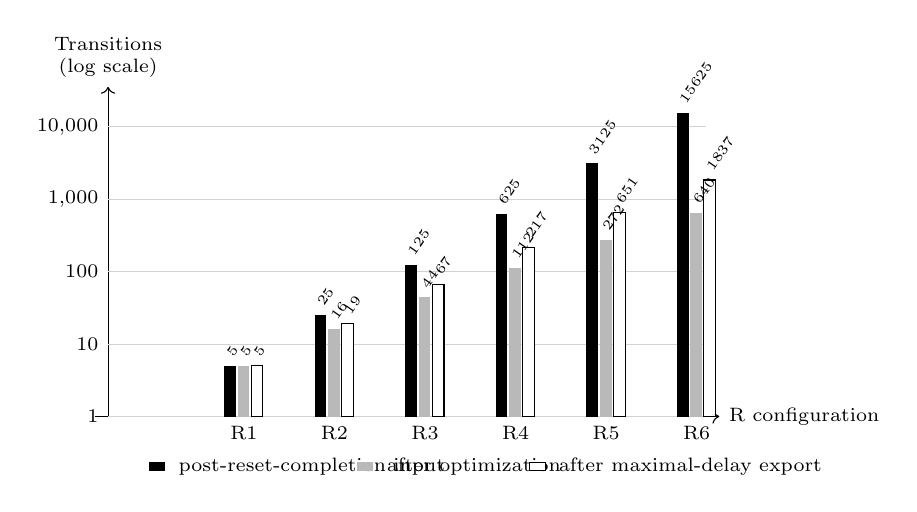
\begin{tikzpicture}[x=1.15cm,y=0.92cm,font=\scriptsize]
  % Vertical positions encode log10(edge count); the labelled y ticks are
  % 1, 10, 100, 1,000, and 10,000 transitions.
  \draw[->] (0.1,0) -- (7.0,0) node[right] {R configuration};
  \draw[->] (0.25,0) -- (0.25,4.55) node[above,align=center]
    {Transitions\\(log scale)};
  \foreach \y/\lab in {0/1,1/10,2/100,3/1{,}000,4/10{,}000} {
    \draw[gray!35] (0.25,\y) -- (6.85,\y);
    \node[left] at (0.25,\y) {\lab};
  }
  % Bars use log10(value) as height. Values above bars are exact counts.
  \foreach \x/\vin/\hin/\vopt/\hopt/\vexp/\hexp in {
    1/5/0.699/5/0.699/5/0.699,
    2/25/1.398/16/1.204/19/1.279,
    3/125/2.097/44/1.643/67/1.826,
    4/625/2.796/112/2.049/217/2.336,
    5/3125/3.494/272/2.435/651/2.814,
    6/15625/4.194/640/2.806/1837/3.264
  } {
    \pgfmathsetmacro{\xc}{\x+0.75}
    \pgfmathsetmacro{\xa}{\xc-0.22}
    \pgfmathsetmacro{\xb}{\xc-0.07}
    \pgfmathsetmacro{\xd}{\xc+0.08}
    \fill[black] (\xa,0) rectangle +(0.13,\hin);
    \fill[gray!55] (\xb,0) rectangle +(0.13,\hopt);
    \fill[white] (\xd,0) rectangle +(0.13,\hexp);
    \draw (\xd,0) rectangle +(0.13,\hexp);
    \node[rotate=55,anchor=west,font=\tiny] at (\xa,\hin+0.04) {\vin};
    \node[rotate=55,anchor=west,font=\tiny] at (\xb,\hopt+0.04) {\vopt};
    \node[rotate=55,anchor=west,font=\tiny] at (\xd,\hexp+0.04) {\vexp};
    \node[below] at (\xc,0) {R\x};
  }
  \fill[black] (0.7,-0.75) rectangle +(0.18,0.12);
  \node[right] at (0.92,-0.69) {post-reset-completion input};
  \fill[gray!55] (3.0,-0.75) rectangle +(0.18,0.12);
  \node[right] at (3.22,-0.69) {after optimization};
  \fill[white] (4.9,-0.75) rectangle +(0.18,0.12);
  \draw (4.9,-0.75) rectangle +(0.18,0.12);
  \node[right] at (5.12,-0.69) {after maximal-delay export};
\end{tikzpicture}

\caption{Post-reset-completion input, optimized TBA, and maximal-delay
explicit export for R1--R6. The logarithmic vertical axis makes the R6
concentration visible. These are positive forms measured with Spot level \texttt{small} and the implementation before the speedups (R7 and R8 did not complete); the counts are five-run medians, and
Comp. (the post-reset-completion input) is the optimizer boundary, regardless of whether an upstream
Spot count happens to match it.}
\label{fig:R-transition-counts}
\end{figure*}

\subsection{Optimization effects on the generated group}
In R6, Spot emits 64 states and 15,625 cube-split transitions. The recorded
post-reset-completion optimizer input also has 64 locations and 15,625
transitions; the equality of these two edge counts is specific to R6, and the
Comp. column is the authoritative optimizer boundary. Six optimization
rounds reduce the transition relation to 640 edges and retain six clocks.
Export then produces 1,837 explicit edges, 63 invariant-bearing locations,
and 3,360 clock-difference guard occurrences; symbolic grouping represents
the output with 448 transitions. The larger explicit edge count results from
splitting disjunctive guards and adding entry conditions for invariant copies.
It measures the cost of the target representation, not a reversal of the
optimizer's reduction. In the fresh run, median optimizer and export times
are 17.807 s and 10.666 s, respectively; these are times of the build before the verified speedups of article Section~\ref{sec:speedups}, with which the optimization of the positive form of R6 takes 0.29~s. Figure~\ref{fig:R-transition-counts} shows the concentration on R6. The generated-group table separately reports the
stage after reset completion so that upstream processing is not folded into
these optimizer measurements.

The same distinction matters for the other generated inputs. For example,
F11 starts from its actual four-location, seven-transition, two-clock TBA
after reset completion; two rounds leave three locations and four
transitions and remove one clock. Two locations have the same loop and the
same exit on $p$ to the accepting location, except that the exit of the first
also carries $x\ge2$; the second is entered only when $x\ge2$ holds and $x$ is
not reset afterwards. They are merged because the guards are compared under
that entry invariant, which equality of guards cannot do. N8 spends most of its end-to-end time in Spot,
whereas its recorded optimizer and exporter stages take 0.33 s and 0.70 s.
These cases show that the optimizer's cost depends on its input relation and
that the upstream producer can dominate total tool time. They do not support
a general runtime or size bound. The runs of this subsection used the former default, Spot level \texttt{small}.
The tool's default is now the automatic mode of article Section~\ref{sec:spot-level};
with level \texttt{low} N8 (positive form) takes 11.6 s instead of 98.3 s, and
the total over the 29 completed configurations falls from 152 s to 58 s (one
run against the five-run medians); optimized sizes are identical except for F5
and F6 (25 to 27 symbolic transitions). The optimizer, the export and the
initial-value check were since made faster by verified rewritings
(article Section~\ref{sec:speedups}), so the timings of the table are those of the
earlier implementation.



\section{Contract table and related-work scope comparison}
\begin{table*}[t]
\centering
\caption{Contract of the verified optimization and export pipeline. The
explicit and symbolic outputs preserve the timed-word language of the TBA
provided to the Rocq interface.}
\label{tab:export-contract}
\small
\begin{tabular}{@{}p{0.22\textwidth}p{0.70\textwidth}@{}}
\toprule
Aspect & Guaranteed result\\
\midrule
Timed-word language & Preserved by every optimization round and by complete export under the development's existential initial-clock semantics.\\
Explicit guards & Conjunctions of event literals and clock comparisons; export may introduce clock-difference comparisons in entry conditions.\\
Location invariants & Conjunctions of non-strict clock upper bounds.\\
Symbolic output & Groups transitions with the same source, target, and reset set under Boolean labels; the symbolic automaton also preserves acceptance.\\
Input adapter & A third-party parser or conversion into the Rocq TBA representation requires a separate correspondence proof to join the verified boundary.\\
\bottomrule
\end{tabular}
\end{table*}

\begin{table*}[t]
\centering
\caption{Scope comparison with representative prior work. ``Not reported'' means not stated in the cited source, not that no related result exists.}
\label{tab:related-work}
\small
\setlength{\tabcolsep}{3pt}
\begin{tabular}{@{}>{\raggedright\arraybackslash}p{0.17\textwidth}>{\raggedright\arraybackslash}p{0.26\textwidth}>{\raggedright\arraybackslash}p{0.34\textwidth}>{\raggedright\arraybackslash}p{0.19\textwidth}@{}}
\toprule
Prior work & Method and setting & Stated guarantee and mechanization & Difference from this paper\\
\midrule
Daws--Yovine~\cite{daws_yovine_rtss1996} & Active-clock reduction and equal-clock merging in timed automata & Algorithmic reduction with case studies; proof-assistant mechanization not reported & Prior clock reduction; no generic TBA pipeline theorem\\
Guha--Narayan--Arun-Kumar~\cite{guha_narayan_arunkumar_concur2014} & Minimum-clock timed-bisimilar automaton & Least clock count; doubly exponential construction; mechanization not reported & Stronger minimization objective, not verified passes/export\\
Yalcinkaya--Aydin Gol~\cite{yalcinkaya_aydin_gol_formalise2019} & Position-based reduction preserving design parameters & Timed bisimilarity and measured clock reduction; mechanization not reported & Direct clock-reduction prior art; this work verifies a composed pipeline\\
Badban--Leue--Smaus~\cite{badban_etal_wing2010} & CIPM invariant generation and idle-transition pruning; split discussed as a direction & Predicate-abstraction method; no split theorem or mechanization reported & Relevant disjunction problem, not generic TBA split preservation\\
De Wulf--Doyen--Raskin~\cite{de_wulf_doyen_raskin_fm2005} & AASAP phase copies, watcher product, multirectangular predicates & Safety equivalence for specialized encoding; mechanization not reported & Phase copies, not one-copy-per-disjunct TBA normalization\\
Bodeveix--Filali~\cite{[BF03]} & Per-disjunct split of UPPAAL disjunctive invariants & Informal; PVS proof announced, ongoing & Prior splitting; no priority claim\\
Wimmer--Lammich / MUNTA~\cite{munta_tacas18,munta_formats19} & Timed-automata reachability checking & Verified checker and executable refinement in Isabelle/HOL & Proves analysis, not TBA optimization/export\\
Wimmer--Herbreteau--van de Pol~\cite{wimmer_herbreteau_vandepol_formats2020} & Timed B\"uchi emptiness certificates & Sound, complete certificate checking in Isabelle/HOL & Verifies checking, not automaton transformation\\
This paper & Iterated optimizer, two split policies, conjunctive explicit/symbolic export & Rocq language preservation for each finite round/export and target-shape theorems & Every TBA of the formula-indexed clock interface; excludes adapters and XML\\
\bottomrule
\end{tabular}
\end{table*}


\section{Generated continuation example}
Figure~\ref{fig:R2-generated} follows an actual current tool-generated automaton from the reset-completion boundary through optimization and export. It does not repeat the upstream MTL translation. In this instance, two optimization rounds remove nine transitions; export adds three explicit transitions while producing the required conjunctive internal shape.

\begin{figure*}[t]
\centering
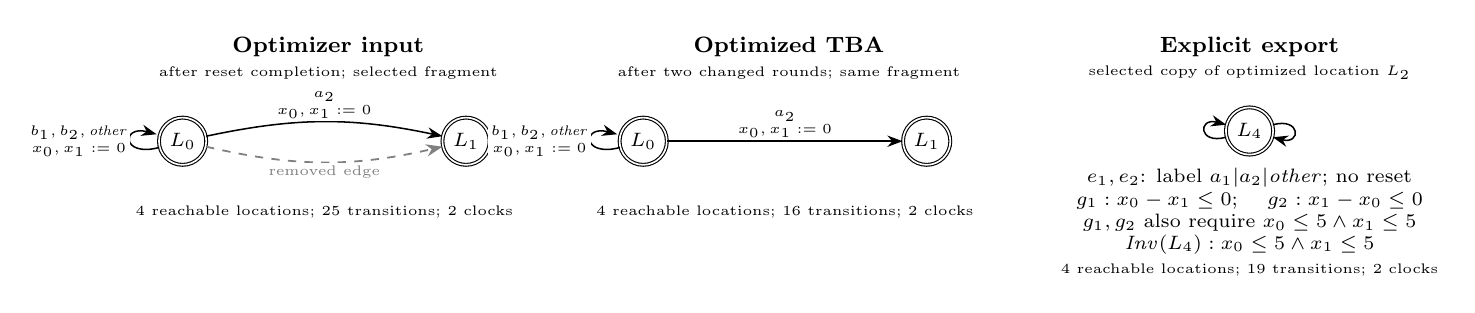
\begin{tikzpicture}[
  state/.style={circle,double,draw,minimum size=6mm,inner sep=1pt,font=\scriptsize},
  edge/.style={->,>=Stealth,line width=0.55pt},
  removed/.style={->,>=Stealth,dashed,gray,line width=0.65pt},
  lab/.style={font=\tiny,align=center,fill=white,inner sep=1pt},
  title/.style={font=\footnotesize\bfseries,align=center},
  small/.style={font=\tiny,align=center},
  detail/.style={font=\scriptsize,align=center}
]
% Each panel is a selected subgraph of the corresponding saved full automaton.
\begin{scope}[xshift=0cm]
  \node[title] at (2.6,2.05) {Optimizer input};
  \node[small] at (2.6,1.72) {after reset completion; selected fragment};
  \node[state] (i0) at (0.75,0.85) {$L_0$};
  \node[state] (i1) at (4.35,0.85) {$L_1$};
  \draw[edge] (i0) edge[loop left] node[lab,left]
    {$b_1,b_2,\mathit{other}$\\$x_0,x_1:=0$} (i0);
  \draw[edge] (i0) to[bend left=12] node[lab,above]
    {$a_2$\\$x_0,x_1:=0$} (i1);
  \draw[removed] (i0) to[bend right=13] node[lab,below]
    {removed edge} (i1);
  \node[small] at (2.55,-0.05)
    {$4$ reachable locations; $25$ transitions; $2$ clocks};
\end{scope}
\begin{scope}[xshift=5.85cm]
  \node[title] at (2.6,2.05) {Optimized TBA};
  \node[small] at (2.6,1.72) {after two changed rounds; same fragment};
  \node[state] (o0) at (0.75,0.85) {$L_0$};
  \node[state] (o1) at (4.35,0.85) {$L_1$};
  \draw[edge] (o0) edge[loop left] node[lab,left]
    {$b_1,b_2,\mathit{other}$\\$x_0,x_1:=0$} (o0);
  \draw[edge] (o0) -- node[lab,above]
    {$a_2$\\$x_0,x_1:=0$} (o1);
  \node[small] at (2.55,-0.05)
    {$4$ reachable locations; $16$ transitions; $2$ clocks};
\end{scope}
\begin{scope}[xshift=11.7cm]
  \node[title] at (2.6,2.05) {Explicit export};
  \node[small] at (2.6,1.72) {selected copy of optimized location $L_2$};
  \node[state] (e4) at (2.6,0.98) {$L_4$};
  % Separate the two loop arcs from their longer guard descriptions.
  \draw[edge] (e4) edge[loop left,looseness=6] (e4);
  \draw[edge] (e4) edge[loop right,looseness=6] (e4);
  \node[detail] at (2.6,0.39)
    {$e_1,e_2$: label $a_1|a_2|\mathit{other}$; no reset};
  \node[detail] at (2.6,0.10)
    {$g_1:x_0-x_1\leq0$; \quad $g_2:x_1-x_0\leq0$};
  \node[detail] at (2.6,-0.19)
    {$g_1,g_2$ also require $x_0\leq5\land x_1\leq5$};
  \node[detail] at (2.6,-0.46)
    {$\mathit{Inv}(L_4):x_0\leq5\land x_1\leq5$};
  \node[small] at (2.6,-0.78)
    {$4$ reachable locations; $19$ transitions; $2$ clocks};
\end{scope}
\end{tikzpicture}

\caption{Selected subgraphs from the actual generated R2 files. The dashed input edge is absent after optimization; only one of the nine removed transitions is shown. The first two panels show a retained edge and loop. The export panel follows the optimized $L_2$ loop to its $L_4$ copy, where one source loop becomes two conjunctive-guard loops. The annotations list their diagonal atoms, shared unary bounds, and invariant. Counts below summarize the complete automata: reachable locations, transitions, and active clocks. The internal output-shape guarantee is proved in Rocq; the displayed graph and counts are measurements.}
\label{fig:R2-generated}
\end{figure*}


\section{Additional evaluation details and tables}\label{sec:eval-extra}
% Material moved from the article to keep it within the page guidance.
\subsection{Generation time on deep nests: profile and the Spot-level trade-off}
\label{sec:deep-nests}
\emph{Where the time goes on deep nests.} A profile of Spot on the simplified
formula of N7 (12.9~s of processor time, 43~MB) attributes 79\% of its time to
its BDD library and 16\% to the rest of Spot. None of the options of
\texttt{spot-x(7)} that we tried (implication-based formula simplification,
formula splitting, SCC filtering, explicit iteration over valuations, Boolean
relabeling, branching postponement) changed the time beyond the run-to-run
spread, and compositional suspension doubled it. On this input the cost appears to lie in the formula
that the verified translation hands to Spot: a bounded eventuality repeats
the translation of its operand three times, so the formula has size $3^k$ in the
nesting depth $k$ (the proposition $p_7$ occurs $2{,}187=3^7$ times in the
formula of N7). Spot's time grows by a factor of about 16 per level while its
output (129 states and 4{,}623 edges at seven levels) grows by about 3.5. On N7,
Spot alone (10--13~s) takes about as long as CASAAL's whole translation
(11.3~s), and the rest of our chain takes about 5~s. On N7 the difference therefore lies in
the replaceable front end (Section~\ref{sec:modular}) and not in the verified
optimization and export; we did not profile N8.

\emph{Why the default is a trade-off.} Against the better explicit setting,
automatic mode loses 0.6~s on N5 (where \texttt{low} is simply the slower
setting), 5.3~s on N6 and 7.0~s on N7 (the 5~s of the abandoned \texttt{low}
attempt plus run-to-run variation of the second run), and it avoids the
minutes that \texttt{low} alone needs on N7 (393~s in a separate run) and the
more than 900~s it needs on N8. On the conjunctions it is never
worse than the former default \texttt{small}, which needs 41~s on seven
responses and fails on eight. On the \emph{positive} forms, which one would give
to a model checker as an assumption, automatic mode costs little: seven
conjoined bounded responses take 14.0~s with \texttt{low}, 8.7~s with
\texttt{any} and 14.3~s in automatic mode, and eight take 89.9~s in automatic
mode, where neither explicit setting finished within the 30~s limit of the
earlier comparison; CASAAL's own times on the positive forms were not measured.
On mixed formulas, nested chains conjoined with plain responses
(Section~\ref{sec:spot-level}), \texttt{any} is at worst 7.7~s where \texttt{low}
needs 0.3~s, which automatic mode avoids by trying \texttt{low} first, and
\texttt{low} exceeds 30~s on nested conjunctions of depth five where \texttt{any}
needs 0.2~s, which automatic mode reaches after its budget.


\subsection{TChecker stored states on the 20 completed products}
Article Section~\ref{sec:casaal-tck} describes the setup and the totals; this is the full table.
\begin{table}[tp]
\centering
\caption{States stored by TChecker (\texttt{tck-liveness}, \texttt{couvscc}) on the product of the negated requirement with a reference system, for the 20 patterns where both runs completed (the product is empty, so it is explored completely and the count does not depend on the exploration order). The reference system is the automaton of the requirement itself, exported by our tool with the diagonal-free all-copy policy, because TChecker rejects diagonal guards. Columns: CASAAL's automaton, our optimized automaton, and ours with the optimizer disabled (\texttt{-n 0}).}
\label{tab:casaal-tck}
\scriptsize
\begin{tabular}{@{}lrrr@{}}
\toprule
Pattern & CASAAL & Ours & Ours, \texttt{-n 0} \\
\midrule
F1 & 461 & 280 & 280 \\
F2 & 3 & 3 & 3 \\
F3b & 3 & 3 & 3 \\
F4 & 266 & 196 & 196 \\
F5 & 459 & 228 & 228 \\
F6 & 521 & 254 & 254 \\
F7 & 652 & 280 & 280 \\
F8 & 76 & 9 & 9 \\
F9 & 191 & 191 & 191 \\
F10 & 1,269 & 1,188 & 1,188 \\
F11 & 69 & 67 & 67 \\
F12 & 2,497 & 1,688 & 1,688 \\
F14 & 6,900 & 3,441 & 3,441 \\
N1 & 48 & 48 & 48 \\
N2 & 967 & 967 & 967 \\
N3 & 22,885 & 22,885 & 22,885 \\
N4 & 498,087 & 498,087 & 498,087 \\
R1 & 461 & 280 & 280 \\
R2 & 21,017 & 7,513 & 7,513 \\
R3 & 674,698 & 168,484 & 168,484 \\
\midrule
Total & 1,231,530 & 706,092 & 706,092 \\
\bottomrule
\end{tabular}
\end{table}


\subsection{Positive-form workload}
\begin{table}[tp]
\centering
\caption{TChecker stored states on the positive forms of the bounded responses with the violating system, all-copy export. ``Inv.\ removed'' deletes the location invariants of our automaton; ``script'' is the unverified invariant script; ``conv.'' is CASAAL's automaton converted to location acceptance and passed through our export (not completed on R5).}
\label{tab:baseline-posbad}
\small
\begin{tabular}{@{}lrrrrr@{}}
\toprule
Requirement & ours & ours, inv. removed & CASAAL & CASAAL + script & CASAAL conv. \\
\midrule
R1 & 48 & 52 & 52 & 48 & 48 \\
R2 & 48 & 52 & 433 & 375 & 375 \\
R3 & 48 & 52 & 4{,}225 & 3{,}439 & 3{,}439 \\
R4 & 48 & 52 & 44{,}389 & 34{,}107 & 34{,}107 \\
R5 & 48 & 52 & 485{,}833 & 353{,}959 & -- \\
\bottomrule
\end{tabular}

\end{table}
\subsection{UPPAAL, model checking and agreement of the verdicts}
\label{sec:uppaal-check}
\begin{table}[tp]
\centering
\caption{UPPAAL~5.0.0, breadth-first search with default extrapolation, on the negated requirement composed with a system, for the products on which the times differ. Stored states are identical in all seven variants; times are medians of three runs including process start; the last column gives the number of explicit property edges of ours and of CASAAL's automaton.}
\label{tab:uppaal}
\small
\begin{adjustbox}{max width=\textwidth}\begin{tabular}{llrrrrrr}
\toprule
Req. & System & Stored & \multicolumn{4}{c}{Time (s)} & Prop. edges \\
\cmidrule(lr){4-7}
 & & (all variants) & ours & ours all-copy & CASAAL & CASAAL+export & ours/CASAAL \\
\midrule
R3 & par-ok & 49 & 0.088 & 0.084 & 0.084 & 0.088 & 56/93 \\
R4 & par-ok & 261 & 0.093 & 0.098 & 0.100 & 0.105 & 90/156 \\
R5 & par-ok & 1631 & 0.166 & 0.171 & 0.251 & 0.207 & 132/235 \\
R6 & par-ok & 11743 & 1.277 & 1.520 & 3.473 & 3.629 & 182/330 \\
N4 & free & 17 & 0.105 & 0.098 & 0.119 & 0.124 & 356/549 \\
N5 & free & 33 & 0.188 & 0.195 & 0.285 & 0.278 & 1275/2063 \\
\bottomrule
\end{tabular}\end{adjustbox}

\end{table}
We generated 311 UPPAAL~5.0.0 models: the negated requirement in seven variants (ours with the default export, with \texttt{-n 0} and with the all-copy export; CASAAL's automaton converted to location acceptance, plain and passed through our export in the same three ways), composed with several systems (a single request/response system, parallel request/response components with their own clocks, a sporadic emitter and a free system). The query is reachability of the accepting sink of the negated safety requirement, not B\"uchi acceptance. All 296 runs with an expected verdict return it, for every variant; the 15 positive-form runs check only that UPPAAL reads the default maximal-delay export, which contains diagonal constraints.
On full explorations the number of stored states is identical in all seven variants on every full exploration except F5 and F8 (3 and 2 states for ours, 4 and 4 for CASAAL's, the smaller translation). Where times differ, they follow the number of explicit property edges: on R6 with parallel components ours needs 1.3~s against 3.5~s for CASAAL (182 edges against 330), and CASAAL's automaton passed through our export is as slow as CASAAL's own (3.6~s), so neither the export nor the optimizer is responsible. Table~\ref{tab:uppaal} lists the products on which the times differ. The negated automata of F1--F9, R1--R6 and N1--N3 have no location invariant in any variant. These are checks on small systems and are single reachability queries; they show that the exported models are usable in UPPAAL and give the same verdicts, not a general speedup.

For timed liveness, which UPPAAL does not decide, we reran the separate TChecker case with and without the optimizer on the same system, property automaton and settings. On ``responds within 4 units'' both runs store 77 states and on ``may remain busy forever'' both store 15; the exported XML and the product automata are byte-identical within each pair, so these examples show neither a speedup nor a regression. XML printing, the adapter and the format correspondence remain outside the mechanized interface.

\subsection{Differential test against an independent judge}
\label{sec:differential}
\begin{table}[tp]
\centering
\caption{Agreement of the automata with an independent evaluator of the MTL semantics on random ultimately periodic timed words (both polarities of each formula). A disagreement is a word on which the automaton and the evaluator differ.}
\label{tab:differential}
\small
\begin{tabular}{@{}llrrr@{}}
\toprule
Set & Automaton under test & Formulas & Word checks & Disagreements \\
\midrule
\multirow{3}{*}{22 benchmark patterns, 20{,}000 words each} & mtl2tba (default export) & 22 & 880{,}000 & 0 \\
 & mtl2tba (all-copy export) & 22 & 880{,}000 & 0 \\
 & CASAAL & 20 & 800{,}000 & 0 \\
\midrule
\multirow{3}{*}{100 random formulas, 6{,}000 words each} & mtl2tba (default export) & 100 & 1{,}200{,}000 & 0 \\
 & mtl2tba (all-copy export) & 100 & 1{,}200{,}000 & 0 \\
 & CASAAL & 100 & 1{,}200{,}000 & 0 \\
\bottomrule
\end{tabular}

\end{table}
To check the automata of both translators against the semantics, not only against each other, we wrote an independent evaluator of the pointwise MTL semantics, transcribed from the Rocq definition of satisfaction, and acceptance evaluators for the UPPAAL XML of our tool (including diagonal guards and invariants) and for CASAAL's DOT output. We drew ultimately periodic timed words with strictly increasing timestamps in multiples of one half, at most nine positions, with delays chosen so that the interval bounds of the formula are hit exactly and one half-unit on either side. On 22 benchmark patterns (20{,}000 words each) and 100 random formulas (6{,}000 words each), in both polarities, the automata of our tool (default and all-copy exports) and of CASAAL accept exactly the words that the evaluator accepts (Table~\ref{tab:differential}, 5{,}960{,}000 word checks, no disagreement). CASAAL has no pointwise next operator, so F3 and F13 are checked for our tool only. The evaluator itself is tested: it rejects 11 of 13 and 7 of 7 deliberately wrong formulas for our tool and for CASAAL. The test finds no bug in either tool; it is agreement on a finite sample of a restricted word class (first event not at time zero, delays multiples of one half), not a proof for either.

\subsection{Seeded defects: what testing misses and the proofs reject}
\label{sec:mutation}
\begin{table}[tp]
\centering
\caption{Seeded defects in the extracted optimizer and exporter. T1: number of the 380 runs whose output differs from the unmutated tool. T2: index of the first random word on which the language test finds a difference, if any. ``Equivalent'' means no language change was found; M17 is argued, not proved.}
\label{tab:mutants}
\small
\begin{adjustbox}{max width=\textwidth}\begin{tabular}{@{}lp{0.34\textwidth}rrrp{0.13\textwidth}l@{}}
\toprule
Mutant & Seeded defect (pass) & T1 & T2 first word & Fuzz & Outcome of the tests & Rocq \\
\midrule
M01 & closed bound 0 on a just-reset clock & 0 & \textemdash{} & 44/234 & missed by T1, T2 & rejected \\
M02 & invariant from min, not max, of branch bounds & 30 & 44 & 154/428 & caught & rejected \\
M03 & x$\ge$2, x$\le$2 always empty (strictness ignored) & 120 & 0 & 1940/3456 & caught & rejected \\
M04 & lower-bound tests ignored for clock liveness & 104 & 0 & 918/1650 & caught & rejected \\
M05 & normalization before dead-reset removal omitted & 78 & \textemdash{} & 0/1116 & no change found & rejected \\
M06 & guard $x>0$ treated as trivially true & 38 & 0 & 770/1284 & caught & rejected \\
M07 & clocks merged without equal reset sets & 14 & 0 & 10/32 & caught & rejected \\
M08 & entry into initial location not excluded & 0 & \textemdash{} & 0/4 & no change found & rejected \\
M09 & accepting and non-accepting locations merged & 6 & 0 & 56/116 & caught & rejected \\
M10 & resets ignored in simulation test & 0 & \textemdash{} & 2/4 & missed by T1, T2 & rejected \\
M11 & parallel transitions merged without comparing resets & 62 & 1 & 184/850 & caught & rejected \\
M12 & complement of $x<c$ taken as $x>c$ & 0 & \textemdash{} & 0/0 & \textbf{missed by all tests} & rejected \\
M13 & entry lower bound from max, not min & 88 & 0 & 1616/2098 & caught & rejected \\
M14 & split copies entered the wrong way round & 15 & 0 & 93/195 & caught & rejected \\
M15 & entry condition not updated for resets & 40 & 0 & 263/462 & caught & rejected \\
M16 & reset clock with $x\le0$ judged false & 0 & \textemdash{} & 31/82 & missed by T1, T2 & rejected \\
M17 & implication direction in disjunct pruning & 1 & \textemdash{} & 5/29 & missed by T1, T2 & rejected \\
M18 & invariants ignored when merging exported locations & 8 & 84 & 36/328 & caught & rejected \\
M19 & initial location pruned as unreachable & 376 & 0 & 6000/6000 & caught & rejected \\
M20 & $x\le u$ taken to imply $x<w$ for $u\le w$ & 24 & 40 & 43/220 & caught & rejected \\
M21 & safety check of dead-reset pass removed & 0 & \textemdash{} & 0/0 & no change found & rejected \\
M22 & weaker bound for conjunctive guard & 0 & \textemdash{} & 0/84 & no change found & rejected \\
\bottomrule
\end{tabular}\end{adjustbox}

\end{table}
\begin{table}[tp]
\centering
\caption{The same mistakes applied to the Rocq definitions: lemma on which the development first fails to compile. The four survivors of Table~\ref{tab:mutants} are M01, M10, M12 and M16; M13, M14 and M19 are further mutants.}
\label{tab:rocq-rejection}
\small
\begin{tabular}{@{}llr@{}}
\toprule
Mutant & First failing lemma & Time (s) \\
\midrule
M01 & \texttt{inv\_guard\_w\_eq} & 4.7 \\
M10 & \texttt{sim\_spec} & 3.8 \\
M12 & \texttt{compl\_cases} & 4.8 \\
M16 & \texttt{const\_true\_spec} & 3.0 \\
M17 & \texttt{insert\_g\_holds} & 4.1 \\
\midrule
M02 & \texttt{max\_all\_ge} & 9.1 \\
M03 & \texttt{contradictory\_bounds\_sound} & 2.7 \\
M04 & \texttt{rename\_item\_holds} & 3.2 \\
M05 & \texttt{optimize\_step\_accepts} & 5.4 \\
M06 & \texttt{trivial\_c\_sound} & 3.8 \\
M07 & \texttt{mergeable\_b\_sound} & 2.8 \\
M08 & \texttt{mergeable\_b\_sound} & 3.3 \\
M09 & \texttt{states\_mergeable\_fast\_eq} & 4.3 \\
M11 & \texttt{same\_ends\_spec} & 4.6 \\
M13 & \texttt{min\_all\_le} & 1.8 \\
M14 & \texttt{notlonger\_complete} & 2.5 \\
M15 & \texttt{split\_trans\_in} & 3.1 \\
M18 & \texttt{dmerge\_states\_ext} & 4.7 \\
M19 & \texttt{dprune\_accepts} & 7.7 \\
M20 & \texttt{implies\_c\_sound} & 2.2 \\
M21 & \texttt{remove\_dead\_resets\_clock\_fast\_eq} & 3.5 \\
M22 & \texttt{ub\_guard\_sound} & 1.9 \\
\bottomrule
\end{tabular}

\end{table}
The agreement above shows that the tools are correct on the sample, not what the proofs add. To measure that, we seeded 22 plausible defects, one at a time, in a scratch copy of the extracted optimizer and exporter (Table~\ref{tab:mutants}; for instance a strict instead of non-strict test at the bound zero, a reset set not compared when two locations are merged, the complement of $x<c$ taken as $x>c$). Each mutant was tested in two ways: by comparing its output with that of the unmutated tool on the benchmark and the corpus of 148 generated automata, and by testing, for 100{,}000 random words per input, whether the output automaton accepts the words of its input.

Seventeen of the 22 mutants change the language of some automaton; the other five do not (M05 changes the output but not the language; M08, M21 and M22 change neither; M17 reverses an implication that we argued is harmless, without proving it). The word-level test finds 13 of the 17. Four, M01, M10, M12 and M16, are not found by any test: the output comparison is blind to them because the benchmark never reaches the defect, and the word test, which fails to notice even a single dropped transition in 36\% of our controls, does not hit the few words that separate the languages. For each of the four we built an automaton on which the mutant's language differs (for M01, 852 accepted sample words become none), so these are real language changes that a test of this kind misses. The test oracle is itself unverified code, and a stronger test may find some of them.

We then applied the same mistakes to the Rocq definitions in a scratch copy of the development (control: the unmutated copy compiles in about 43 s with the four standard axioms). All four survivors are rejected by Rocq within 3 to 5 seconds at a named lemma (Table~\ref{tab:rocq-rejection}), as are the three further mutants we tried (M13, M14, M19); we did not run the other 15. The rejection is at the lemma that ties the implementation to its specification (for M01, against the specification function of the invariants), so the check is only as strong as that specification: a mutation that changed implementation and specification together would pass. These results make a bounded claim: for these defects in this code, a test of 100{,}000 words did not find four that the development rejects. They do not show that CASAAL contains such defects, and CASAAL may well be correct.


\subsection{Generated group: setup details and aggregates}
This section evaluates the whole translation from an MTL requirement to the
automaton given to a timed model checker, and the optimization passes inside
it. It asks four questions. First, how does the translation compare, tool to
tool, with an independent translator, CASAAL, in the size of the automaton, in
generation time and in the cost the automaton imposes on a timed model checker
(Section~\ref{sec:casaal-eval})? Second, which structures do the verified
optimization passes remove or simplify, and how much of the difference to
CASAAL do they explain? Third, what size and timing cost does conversion to
conjunctive guards and invariants add? Fourth, do the packaged system checks
behave as intended? Internal output shape is a Rocq theorem; external checker
verdicts, sizes and times are experimental evidence. The matched TChecker
cases below show unchanged exploration on systems whose exported models are
byte-identical before and after optimization; they do not establish a general
cost improvement.

We retain the 31-attempt F/R/N benchmark as an upstream-generated
group. The optimizer input is the automaton after reset completion, shown as
Comp. in Supplement Table~\ref{tab:optimizer-benchmarks}. Of the 31 attempted
configurations, 29 completed this upstream stage and supplied an optimizer
input; R7 and R8 timed out before the measured boundary (with the later
implementation of Section~\ref{sec:speedups}, their positive forms complete in
14 s and 90 s). Formula rewriting, Spot
configuration, cube expansion, relaxation, and reset completion happen
upstream; their effects are not credited to the optimizer. The runs use the
tool's default front end, which before translation rewrites
$\Box\Diamond_{\ge d}\varphi$ into $\Box\Diamond\varphi$ and
$\Diamond\Box_{\ge d}\varphi$ into $\Diamond\Box\varphi$, and which replaces
the Until of the clauses of upper-bounded hatted Until by a weak Until. The
end-to-end theorem for this front end is
\path{MTL_to_exported_correct0_recur_weak_with}
(\path{MTL_to_TBA_Recur.v}); the optimizer theorems are unaffected, since
they hold for every input TBA of the interface. Results
are medians of five runs per completed configuration, with a 300~s limit per
attempt, on Ubuntu 26.04/WSL~2, an Intel Core i7-8650U at 1.9~GHz with
11.7~GB of memory, OCaml 5.4.0, Rocq 9.0.1, and Spot 2.16. The generated-group
sizes and times of this section were measured with the Spot level \texttt{small} and
the implementation before the speedups of Section~\ref{sec:speedups}; the run log, machine record, summary
table, and generated automata are preserved under
\path{evaluation/runs/2026-10-14-full-eval-v3/}.
The per-instance table is in Supplement Table~\ref{tab:optimizer-benchmarks}.

Across the 29 completed inputs, the sum of reachable transition counts falls
from 20,204 at the post-reset-completion boundary to 1,500 after optimization
(an aggregate reduction of 92.58\%). Nineteen cases have fewer transitions
and 10 are unchanged. This aggregate is strongly skewed: R6 contributes
14,985 of the 18,704 removed transitions, so the percentage is not a typical
per-instance reduction. Active clocks used in guards or resets sum from 77
to 74; only three cases (F2, F11, F13) reduce this count. The export stage has a different
effect: explicit transitions sum from 1,500 to 3,209, an increase of
113.93\%; six exports grow and 23 have the same count as their optimized
input. Export-size change is reported separately from optimization and is
not counted as an optimization regression.
\begin{table*}[tp]
\centering
\caption{Family aggregates derived from the completed rows of Table~\ref{tab:optimizer-benchmarks}. Edge totals are measured at the post-reset-completion optimizer boundary, after optimization, and after explicit export.}
\label{tab:optimizer-aggregates}
\scriptsize
\setlength{\tabcolsep}{3pt}
\begin{adjustbox}{max width=\textwidth}\begin{tabular}{@{}p{0.22\textwidth}rrrrrr@{}}
\toprule
Group & $n$ & Input $\sum E$ & Opt. $\sum E$ & Reduction & Exp. $\sum E$ & Cases $\downarrow/= /\uparrow$\\
\midrule
F group & 15 & 172 & 126 & 26.74\% & 128 & 7/8/0 \\
bounded-response R group & 6 & 19,530 & 1,089 & 94.42\% & 2,796 & 5/1/0 \\
N group & 8 & 502 & 285 & 43.23\% & 285 & 7/1/0 \\
\bottomrule
\end{tabular}\end{adjustbox}
\end{table*}

The family breakdown shows how concentrated these totals are. The six
completed bounded-response R cases account for 18,441 of the 18,704 removed
transitions (98.59\%); the F and N groups remove 46 and 217, respectively.
The R group's explicit export grows from 1,089 to 2,796 transitions, while
the F group grows by two and the N group is unchanged. Thus the aggregate
optimizer reduction is driven mainly by one bounded-response family, and the
export expansion is a separate representation cost concentrated in that same
family.

Part of this reduction only re-merges the cubes that Spot emits one by one.
With symbolic grouping applied in both runs, the optimizer alone lowers the
symbolic transition count (\texttt{-n 0} against the default) from 704 to 344
(51\%) on the 27 configurations whose unoptimized export completes: from 364
to 216 on F and N, and from 340 to 128 on R1--R4. It is smaller in 17 and
equal in 10 (per-instance rows in \path{evaluation/symbolic_before_after.tsv}). In the recorded runs the unoptimized export of R5 and R6 did not finish
within 300 s, whereas the optimized pipeline completed them in 3.6 s and 39.0 s;
after the verified speedups of Section~\ref{sec:speedups} the unoptimized export
of R5 finishes, with 5,469 explicit transitions against 651 for the optimized one.


\subsection{Matched comparison of the two export policies}
We reran R2--R6 once with each verified split policy while holding the optimized automaton fixed; the optimized TBA DOT files were byte-identical across the two invocations. The table reports explicit-edge counts, diagonal guard atoms and single-run exporter time returned by the tool. All-copy export has no explicit-edge growth beyond the optimized relation and adds no diagonal guards; maximal-delay export adds explicit edges in each case and introduces between 2 and 3,360 diagonal guard atoms per formula (4,464 in total). This is a measured property of this benchmark family, not a general size theorem.
\begin{table*}[tp]
\centering
\caption{Matched maximal-delay and all-copy exports for R2--R6. The two
policies receive byte-identical optimized TBA graphs. Export time is one
observed run per row and policy; it is descriptive and should not be read as
a stable speed ranking.}
\label{tab:generated-export-policy}
\scriptsize
\setlength{\tabcolsep}{4pt}
\begin{tabular}{@{}lrrrrrrr@{}}
\toprule
ID & Optimized $E$ & Max-delay $E$ & All-copy $E$ & Max-delay diagonal atoms & All-copy diagonal atoms & Max-delay time (s) & All-copy time (s)\\
\midrule
R2 & 16 & 19 & 16 & 2 & 0 & 0.002 & 0.005\\
R3 & 44 & 67 & 44 & 30 & 0 & 0.014 & 0.024\\
R4 & 112 & 217 & 112 & 192 & 0 & 0.195 & 0.190\\
R5 & 272 & 651 & 272 & 880 & 0 & 1.319 & 1.052\\
R6 & 640 & 1,837 & 640 & 3,360 & 0 & 9.689 & 9.614\\
\bottomrule
\end{tabular}
\end{table*}

Both policies retain the same reachable location counts, active clock counts and invariant-bearing locations on these runs. Peak RSS of the full tool process, including Spot and optimization, was 17.2/17.3 MB for R2 and 108.5/107.0 MB for R6 (maximal-delay/all-copy); these do not isolate export memory. The observed exporter times have no consistent ordering: all-copy takes longer for R2/R3 and shorter for R4/R5, with similar times for R6.

\subsection{Synthetic suite: interaction cases}
\begin{table*}[tp]
\centering
\caption{Measured direct TBA examples targeting propagation and pass interactions. Transition and clock counts are total records and active clocks. Leave-one-operation-out variants are experimental composites, not separately verified transformations.}
\label{tab:synthetic-interactions}
\scriptsize
\setlength{\tabcolsep}{3pt}
\begin{tabular}{@{}p{0.22\textwidth}cccp{0.39\textwidth}@{}}
\toprule
Case & Input $E/C$ & Full $E/C$ & Rounds & Measured target-pass effect when omitted\\
\midrule
Backward bound tightening & 2/1 & 2/1 & 1 & Incoming guard tightens from $x\leq5$ to $x\leq2$; omitting backward synthesis leaves $x\leq5$.\\
Forward lower-bound propagation & 3/1 & 3/1 & 1 & Entry fact $x\geq2$ is added to the outgoing $q$ edge; edge count is unchanged.\\
Forward contradiction cascade & 7/1 & 4/1 & 2 & Omitting forward propagation or contradiction removal retains 7 edges; the full run removes the $x\leq1$ branch and then prunes its unentered chain.\\
Backward contradiction cascade & 5/1 & 1/0 & 2 & Omitting backward synthesis leaves 2 edges/1 clock; omitting contradiction removal leaves 5/1.\\
Normalization and dead reset & 2/1 & 2/0 & 1 & Normalizing tautological $x\geq0$ enables reset removal; omitting either pass leaves 1 active clock.\\
Synchronous-clock contradiction & 5/2 & 3/1 & 2 & Merging the synchronously reset clocks exposes $x\geq5\land x\leq3$; omitting clock merge or contradiction removal leaves 5 edges/2 clocks.\\
\bottomrule
\end{tabular}
\end{table*}


\section{Random formulas and export policies on every configuration}\label{sec:random}
The 100 random formulas of the translation article (depth at most three, three propositions; \path{evaluation/random_formulas.tsv}) were run through the default pipeline with the optimizer enabled, by \path{evaluation/run_random_opt.sh} (current tool, default automatic Spot mode, limit of 120~s per formula); all 100 complete, the slowest in 0.3~s, and none needs more than three optimization rounds. Over the 100 formulas, the explicit transitions of the optimizer input total 3,980 and those of the optimized automaton 2,366; locations 784 and 638; clocks 160 and 131. The optimizer reduces transitions on 50 formulas, locations on 25 and clocks on 25, and increases none of the three. The exported automaton has 638 locations and 2,391 transitions in total (the maximal-delay export adds difference guards on some formulas). The verified \texttt{init\_free} check succeeds on 96 formulas and fails on four (X38, X65, X84, X100), for which the zero-initial-clock reading of UPPAAL is therefore not covered by the proved condition. A first run with the former default Spot level, whose Spot automata are different, gave 2,507 and 1,509 transitions, 696 and 564 locations, 160 and 128 clocks, reductions on 57, 25 and 26 formulas, and no increase; the qualitative picture is the same. These are size and timing measurements; they do not check language equivalence, which the proofs provide for the optimizer and the export. The per-formula rows are in \path{evaluation/random_opt_nov9.tsv} (current run) and \path{evaluation/random_opt.tsv} (first run).

Table~\ref{tab:export-policies} compares the two export policies on every configuration of the generated benchmark: the maximal-delay export (default) and the separately verified all-copy split (\texttt{-all-copy}), by \path{evaluation/run_export_policies.sh}. The two exports have the same number of invariants on every completed configuration. The all-copy export has exactly the transitions of the optimized automaton and no difference guards. The maximal-delay export has more transitions on F14 and R2--R6 (for example 1,837 against 640 on R6, with 3,360 difference guards) and the same number elsewhere; the totals over the 29 completed configurations are 3,209 and 1,500. R7 and R8 do not complete under either policy within 300~s.

\begin{table}[t]
\centering
\caption{Both export policies on every configuration. Opt.: transitions of the optimized automaton. Max.-delay (default) and all-copy: transitions, invariants, and difference guards of the exported automaton. R7 and R8 do not complete within 300~s.}
\label{tab:export-policies}
\scriptsize\setlength{\tabcolsep}{4pt}
\begin{adjustbox}{max width=\textwidth}\begin{tabular}{@{}lrrrrrrr@{}}
\toprule
ID & Opt. & \multicolumn{3}{c}{Max.-delay} & \multicolumn{3}{c}{All-copy}\\
\cmidrule(lr){3-5}\cmidrule(l){6-8}
& & Trans. & Inv. & Diff. & Trans. & Inv. & Diff.\\
\midrule
F1 & 5 & 5 & 1 & 0 & 5 & 1 & 0\\
F2 & 1 & 1 & 0 & 0 & 1 & 0 & 0\\
F3 & 5 & 5 & 0 & 0 & 5 & 0 & 0\\
F3b & 1 & 1 & 0 & 0 & 1 & 0 & 0\\
F4 & 5 & 5 & 1 & 0 & 5 & 1 & 0\\
F5 & 25 & 25 & 0 & 0 & 25 & 0 & 0\\
F6 & 25 & 25 & 0 & 0 & 25 & 0 & 0\\
F7 & 4 & 4 & 1 & 0 & 4 & 1 & 0\\
F8 & 4 & 4 & 0 & 0 & 4 & 0 & 0\\
F9 & 9 & 9 & 2 & 0 & 9 & 2 & 0\\
F10 & 13 & 13 & 2 & 0 & 13 & 2 & 0\\
F11 & 4 & 4 & 1 & 0 & 4 & 1 & 0\\
F12 & 5 & 5 & 1 & 0 & 5 & 1 & 0\\
F13 & 3 & 3 & 1 & 0 & 3 & 1 & 0\\
F14 & 17 & 19 & 4 & 2 & 17 & 4 & 0\\
R1 & 5 & 5 & 1 & 0 & 5 & 1 & 0\\
R2 & 16 & 19 & 3 & 2 & 16 & 3 & 0\\
R3 & 44 & 67 & 7 & 30 & 44 & 7 & 0\\
R4 & 112 & 217 & 15 & 192 & 112 & 15 & 0\\
R5 & 272 & 651 & 31 & 880 & 272 & 31 & 0\\
R6 & 640 & 1837 & 63 & 3360 & 640 & 63 & 0\\
R7 & -- & -- & -- & -- & -- & -- & --\\
R8 & -- & -- & -- & -- & -- & -- & --\\
N1 & 5 & 5 & 1 & 0 & 5 & 1 & 0\\
N2 & 9 & 9 & 2 & 0 & 9 & 2 & 0\\
N3 & 16 & 16 & 3 & 0 & 16 & 3 & 0\\
N4 & 25 & 25 & 4 & 0 & 25 & 4 & 0\\
N5 & 36 & 36 & 5 & 0 & 36 & 5 & 0\\
N6 & 49 & 49 & 6 & 0 & 49 & 6 & 0\\
N7 & 64 & 64 & 7 & 0 & 64 & 7 & 0\\
N8 & 81 & 81 & 8 & 0 & 81 & 8 & 0\\
\bottomrule
\end{tabular}\end{adjustbox}
\end{table}



\section{Moved from the article: Spot settings, count sensitivity and non-empty products}
\label{sec:spot-level-detail}
This section holds text that the article summarizes: the measurements behind the choice of the Spot level (article Section~\ref{sec:spot-level}), and the checks of how far the verified stages contribute to the TChecker counts and of the verdicts on non-empty products (article Section~\ref{sec:tck-sensitivity}).

\subsection{Choosing the Spot level}
The propositional automaton is produced by \texttt{ltl2tgba -B --<level> [-x <options>] --hoa} and read back by the tool (the reader is outside the proofs). The theorems hold for every automaton that accepts the propositional models of the clocked formula, so neither level nor options affect correctness; they affect running time a great deal and the size of the result little on our benchmark: levels \texttt{small} and \texttt{low} give the same optimized size on every configuration but F5 and F6 (25 against 27 transitions).



Two settings matter. Level \texttt{low} is instantaneous on conjunctions of bounded responses, where \texttt{any} is slow (seven responses, negated: 0.1~s against 11.9~s), and slow on deeply nested bounded eventualities (six levels, negated: 13.9~s against 1.3~s for \texttt{any} on the simplified formula). Spot's simulation-based reduction takes more than half of its time at level \texttt{any} and removed nothing on our inputs; switching it off with \texttt{-x ba-simul=0} cut the time on nested requirements by a factor of 2.8 (seven levels: 28~s to 10~s for Spot alone, same 129 states and 4,623 edges). With that option, \texttt{any} and \texttt{low} give automata of the same size on each of the 57 pattern--polarity pairs where both finish within the limit.



No level is best everywhere and we found no rule on the shape of the formula (a nested chain of depth five conjoined with five responses takes 0.3~s with \texttt{low} and 7.7~s with \texttt{any}; without the responses, \texttt{low} exceeds 30~s at two conjuncts and \texttt{any} needs 0.2~s). The default is therefore an \emph{automatic mode} (\texttt{-spot-level auto}): it runs Spot at level \texttt{low} and, if Spot has not finished after a budget of $b$ seconds (\texttt{-spot-budget}, default 5), stops it and runs level \texttt{any} with \texttt{ba-simul=0} on the formula simplified by the proved simplification \path{ltl_simp_correct}. Both steps are instances of the verified translation and only Spot remains trusted. The fallback costs at most $b$ seconds; the choice depends on a wall-clock measurement, so the level, and with it the run time, can differ between runs and machines.



The mode can be overridden with \texttt{-spot-level}, \texttt{-simp} and \texttt{-spot-x}: for requirements whose conjuncts are all deeply nested chains (depth four or more), \texttt{-simp -spot-level any -spot-x ba-simul=0} skips the budget spent on \texttt{low} (N6: 1.3~s against 6.6~s in automatic mode), and benchmarking should fix the level so that the automaton does not depend on machine speed. On our inputs no other \texttt{spot-x} option than the simulation reductions improved the time, and for plain responses no override is worth its cost. article Section~\ref{sec:casaal-time} reports automatic and manual times side by side.




\subsection{Sensitivity of the TChecker counts}\label{sec:tck-sensitivity-detail}

Three checks bound what the verified stages contribute to these counts.
\emph{Optimizer.} With the optimizer disabled (\texttt{-n 0}), TChecker stores exactly the same
number of states on each of the 20 products, although the optimizer reduces the automaton: from 688 to 461
transitions on N5, from 2{,}737 to 1{,}541 on N6, from 10{,}930 to 5{,}105 on N7 (the size of CASAAL's automata
in each case) and, on the positive form of five conjoined bounded responses, the exported automaton from
5{,}469 to 651 transitions. Running TChecker on the automaton before any pass (the output of reset
completion) gives the same count as on ours on six of seven products tried (F1, F7, R2, R3, N2, N3) and
1{,}790 instead of 1{,}688 on F12.
\emph{Invariants.} Only F10--F12 carry location invariants in our negated automata. Removing
them changes the total from 204{,}564 to 204{,}749, all of it on F10--F12 (and for CASAAL's automata from
204{,}819 to 205{,}004).
\emph{Optimizer on CASAAL's automata.} On every CASAAL automaton that the importer converts (F1--F12,
R1--R8, N1--N5), the optimizer changes nothing: these automata are a fixed point of our passes, which is
consistent with their equal size. A hand-made automaton with redundant guards shrinks under the same
driver, so the importer does not prevent the passes from acting.

\subsection{Non-empty products}

All products above are empty, so they show the size of the state space but not
that the translators agree on a verdict when the system violates the
requirement. We therefore composed the negated automata with two kinds of
system. A \emph{free} system allows every event at every time (strictly
increasing, divergent timestamps): for each of the 20 products, ours (default,
\texttt{-n 0}, invariants removed) and CASAAL's automaton in three variants (with and without an invariant script, and converted and exported) give a
non-empty product, 138 verdicts in all, with no disagreement (F14 cannot be converted).
A \emph{response} system for R1--R3 either answers every request within two
time units or never answers the first one; the products are empty in the first
case and non-empty in the second, for every variant and for both export
policies, with no disagreement (42 verdicts for each case). TChecker stops at
the first violation, so state counts of non-empty products depend on the search
order and are not compared. article Section~\ref{sec:verification-adds} reports the same check
with UPPAAL.



\bibliographystyle{elsarticle-num}
\bibliography{jss_references}
\end{document}
